\documentclass[12pt,a4paper]{report}

\usepackage[utf8]{inputenc}
\usepackage[T1]{fontenc}
\renewcommand{\familydefault}{\sfdefault}
\usepackage{amssymb,amsmath}
\usepackage{epsfig}
\usepackage{multirow}

\usepackage{amssymb}
\usepackage{subfigure}
\usepackage{graphicx}
\usepackage{graphicx,calc}
\graphicspath{ {./figures/} }
\usepackage{caption2}
\usepackage{setspace}
\usepackage{style/ps-macros}
\usepackage{paralist}
\usepackage{rotating}
\usepackage{apacite}
\usepackage[strings]{underscore}
\usepackage[headheight=60pt,tmargin=65pt,headsep=10pt]{geometry}
\usepackage{fancyhdr}
\fancyhead{}
\renewcommand{\headrulewidth}{0pt}
\usepackage{overpic}
\usepackage{xcolor}

\usepackage{url}
\def\UrlBreaks{\do\/\do-}

\usepackage{etoolbox}
\AtBeginEnvironment{quote}{\par\singlespacing\small}

\usepackage{afterpage}
\newcommand\blankpage{
    \null
    \thispagestyle{empty}
    \addtocounter{page}{-1}
    \newpage
    }

\let\chaptername\relax

\setcounter{secnumdepth}{3}    % n - number of sectioning levels
\setcounter{tocdepth}{3}       % up until which sectioning level will be shown in the summary
\setlength{\parskip}{1\baselineskip}

\begin{document}

\thispagestyle{empty}
\addtocounter{page}{-1}
\newgeometry{left=-0.615cm,right=0cm,top=0cm,bottom=0cm}


\includegraphics[height=\paperheight]{figures/Cover_Front}

\restoregeometry

\thispagestyle{empty}
\addtocounter{page}{-1}
\newgeometry{left=7cm,right=2.5cm,top=3cm,bottom=3cm}
\uchyph=0

\begin{figure*}[t!]
    
\includegraphics{figures/HTW_Logo}
\end{figure*}

\mbox{}
\vfill
\vspace{3cm}
\large
\noindent
\textbf{Gamification in Education and Skill Development:\\Implementing Gaming Techniques for Effective\\Learning and Skill Acquisition in Personal Contexts}\\

\normalsize
\noindent
Bachelor Thesis

\vspace{0.6cm}
\small
\noindent
Degree: Game Design\\
Faculty 5 - Gestaltung und Kultur\\

\mbox{}
\vfill
\noindent
submitted by Marlene, Tonnelier - 577261\\
Date: Berlin, 10.03.2024\\
\\
\noindent
First Examiner: Prof. Thomas Bremer\\
Second Examiner: Julia Peters

\restoregeometry
\afterpage{\blankpage}

\thispagestyle{plain}
\addtocounter{page}{-1}
\pagenumbering{gobble}
\newgeometry{left=7cm,right=3cm,top=8cm,bottom=3cm}

\large
\noindent
\textbf{Abstract}\\

\small
This paper is a compilation looking at a general consensus on which gamification elements are considered effective for the development of a gamified application specifically for skill and knowledge acquisition. Keywords like Gamification, Game-Based Learning and Educational Games are compared and differentiated, the benefits of Gamified learning clarified and how the current state of gamification in education is. Furthermore, general design elements in games and elements of learning that can be translated into gamification are analysed, as well as motivators like intrinsic and extrinsic motivation and general reward systems. Finally a list is compiled of the gamification elements considered most effective for this purpose alongside with a few questions that can be asked during the development process of such an application.\\
\\
\\
Keywords: Gamification, Game Design Frameworks, Reward Systems, Skill Acquisition

\restoregeometry
\pagenumbering{arabic}

\fancyfoot[C]{
    \raisebox{-0.5ex-\height}{%
    \begin{overpic}{figures/Footer}
        \put(48,40){\color{white}\thepage}
    \end{overpic}}}

\pagestyle{fancy}

\fancypagestyle{plain}{%
    \fancyheadoffset[R]{3.3cm}
    \fancyfoot[C]{
        \raisebox{-0.5ex-\height}{%
        \begin{overpic}{figures/Footer}
            \put(48,40){\color{white}\thepage}
        \end{overpic}}}

    \fancyhead[R]{
        \setlength{\voffset}{-5cm}
        
\includegraphics{figures/Header}
    }
}

\tableofcontents
\listoffigures
\newpage

\chapter{Introduction}
Gamification in general is a fairly new field of study, especially when it comes to the combination of gamification and education, even more so in non-academic contexts. Individual learning has become accessible to the masses over the recent years due to the development and accessibility of smartphones, their presence permeating every aspect of life, presenting a powerful tool to acquire new knowledge and skills on a private, individual level.

Despite the massive increase in studies in the recent years that try to cover this topic, there is very little consensus on which gaming techniques and elements are seen as effective and universally applicable to gamification tools in general, even less so in learning. This paper compiles the current state of the art of research in this field, especially focussing on the overlap of efficient instructional design and gamification techniques and finally curate a comprehensive list of which gamification elements can universally be implemented in the development of a gamified learning application for private use.
\newpage

\section{Methodology}
Despite the research on the efficacy of gamification not being inexistent, not all authors will focus on evaluating the same elements and the outcome of the same techniques. To best create a compilation of relevant knowledge, this paper focuses on the analysis of Gamification, Game-Based Learning, Educational Games, and different Reward Systems.

Even focusing on the most common themes and keywords, not all of the papers in this compilation will touch every aspect of gamification. To keep this work consistent, a result was only included if it was present in two or more papers; that was considered the bare minimum to analyse the consensus and to explore where authors diverge on their observations.

Given how relatively new the topic of gamification in personal learning contexts is, this compilation also includes results of studies in adjacent topics, like Game-based learning, games in education in general, as well as formal academic education. Although these are not the precise areas that this paper is proposing to analyse, they are close enough and were necessary to create a significant sample of the state of the art. It is expected that with more time and development in the field, more research will be done in the specific area of gamification for individual, independent learning.


\chapter{State of the Art}
No matter the age, culture, social background or ethnicity, people have always loved to play games \cite{framework}.
Saying that games are an attractive medium throughout the population regardless of gender, age, and other social factors is an understatement \cite{mmo}.
The Entertainment Software Association conducted a survey which found that at least 67\% of American head of households play computer or video games on a regular basis and other studies have been done, showing that there is considerable interest and curiosity amongst the learner population to use games and gamified tools for skill aqcuisition purposes due to their known ability to engage players and keep them motivated \cite{engage} \cite{framework}.
Despite their popularity, formal education systems keep a sceptical view towards games in education, doubting their efficiency and painting them in a generally unserious light \cite{lifelong}.

Contrary to how it might be percieved, digital games are not new at all to the field of education. Educational games and Edutainment\footnote{Edutainment according to the Cambridge Dictionary: 'the process of entertaining people at the same time as you are teaching them something, and the products, such as television programmes or software, that do this' \cite{cambridge}} represent 7-9\% of the video game market \cite{engage}.
Current modern pedagological trends in education are a good opportunity to introduce new digital approaches to traditional and long-established teaching methods in order to enhance active learning and encourage new approaches. The ever-increasing use of Information and Communication Technology in learning context reinforces why the time to double down on introducing these approaches is now \cite{edu}.
Additionally to its popularity on smaller scale levels like in schools and in homes, Game-Based Learning has been taken more seriously on a political level as well, the European Union actively supporting and initiating multiple projects on an EU-wide scale like the Elektra Project (2009) - an adventure game designed to keep up with commercial games with a focus on curriculum-related educational purposes by incorporating a sound psychological and pedagogical framework \cite{elektra} - and 80 Days (2009) - a video game inspired by Jules Verne's novel "Around the world in eighty days" with the goal of creating a game that integrates intelligent and pedagogically proven personalisation and provides interactive and individual storytelling \cite{eightydays} \cite{lifelong}.

Many academic papers seem to agree that despite decades of research on games used for educational purposes, there is a considerable lack of appropriate and interesting media and content that engages learners and improve the learning process or add to it. Furthermore, besides the lack of actual good content, there is a notable shortage of guidelines or frameworks for effective educational game design models, causing instructional designers and game designers alike to develop their applications with a trial and error approach \cite{aspects} \cite{framework} \cite{online} \cite{model} \cite{equilibrium}.
One paper claims additionally that another issue that this sector of research has, is the inconsistency in the outcomes of empirical research regarding Gamification in learning environments, leading to inconclusive results about the efficiency of their usage \cite{equilibrium}, however others claim that there are plenty of studies by various researchers that indicate the opposite, showing that many strategies, tactics and methods used in popular gaming can provide valuable lessons and tools for the design of instructional media \cite{engage}.
Despite researching the overall effectiveness of games and gamification in instructional contexts, research has often ignored the actual methods and tactics that popular game design uses to engage their players and how these might be translated to educational game design \cite{engage}.
Past research also mostly focussed on specific game genres and their design, making their finds and suggestions harder to use and implement when the target game genre of the new product differs to the one in the study \cite{model}.

In educational environments as well as in the general environment of skill acquisition, there is a growing demand for the learning materials to be more interactive as well as offer individualisation and customisation of such materials to cater to todays learners needs \cite{aspects}.
Game-Based Learning is already being widely used in childrens education all over the world \cite{aspects} and an increasing number of countries - specifically in northern europe like Norway or Sweden - are implementing a higher focus on digital skills in their education system, routinely using either full games or gamified tools like Quiz-games in their curriculum and teaching methods \cite{domestic}.

Overall, digital games as a means of learning have gained more importance due to changes in modern infrastructure and the society as a whole \cite{lifelong}.
The lives of people of newer generations are significantly more entwined with the digital world, be it at home, in schools or in the workplace, making them so-called "digital natives", adept at navigating the web and other technologies with ease. This, as well as the huge popularity of video and computer games throughout all generations and populations, are reasons as to why new ways of learning have to be discovered and developed to stay up-to-date with the needs, trends and capabilities of individuals in modern society \cite{aspects} \cite{domestic} \cite{online} \cite{framework}.
Due to those ever-changing consumer demands, game designers are continuously looking for new ways and strategies to engage their players \cite{mmo}.

Though there are overarching similarities between commercial games designed with the sole purpose of entertaining the player and games specifically designed for educational purposes, studies make an important distinction between them in their research \cite{domestic}.
Despite both being on the rise in their respective fields and industries, as previously mentioned, e-learning and digital media in the educational field have been under heavy scrutiny by academics and educators alike due to a number of current limitations but it seems that the academic debate about the educational value and potential of such content is decreasing and instead shifting focus towards questions found in the development of such media, namely the cost of development, the complexity and challenges in implementing said media into the curriculum, or how to assure the quality of the learning process \cite{online}.
Since this topic has been gaining notably more momentum in popular debates, a growing number of tools are being created to facilitate the implementation of games and gamification into current learning contexts \cite{online}.

Game-Based Learning and Gamification are models that commonly get seen as a 'cure-all' for the problems of traditional education due to the popularity of gaming in society \cite{traditional}. Although this view is very much blown out of proportion, one can't ignore the aspects that gamified learning can bring to the table. Studies show that educational games provide immersion, motivation and fun, as well as provide content that the user can relate to and that is rooted in reality, teaching 21st century skills all while serving its original purpose \cite{framework}.
There are many studies that show pleasure and fun to be inherent aspects of games, and systems specifically for designing games for a learning environment context use those as core motivators to improve learner's engagement \cite{compare}.

Despite instructional designers and game designers best efforts, educational games often lack the engagement and fidelity that they want to copy from commercial games. Vice versa, commercial games generally fall short on intellectual content that truly teaches subject matters in a constructive and pedagogically sound way.
To create meaningful and effective tools for skill acquisition, it is crucial to find ways to combine the two, pick and choosing which elements of which can enhance the overall performance and utility of the tool to develop powerful and motivating gamification \cite{traditional}.

\section{The bad reputation of Educational Games}
Although the newer generations are avid tech users who navigate the digital world on a daily basis, educational games are associated with negative feelings and are often seen as boring in the best case \cite{model} \cite{domestic}, or outright useless or even damaging in the worst \cite{domestic} \cite{lifelong}.
Critical voices claim that learning through games simply disguises traditional teaching and therefore won't be enjoyable in and of itself in the first place \cite{domestic}.
Additionally, using games within learning contexts usually have somewhat of an unserious flavour to it, especially from the perspective of formal educational systems since games are still percieved as a mere entertainment medium \cite{lifelong}.
Another reason for the bad reputation of educational games might be the ongoing debate whether games in general are harmful to players, for example due to some titles' extreme violence like Call of Duty, published by Activision or the Counter Strike franchise, by Valve Corporation, rendering games unattractive as a medium for learning in school contexts \cite{domestic}.
The question of why no actually good and fun educational games have been developed yet is a widely spread one, and can be traced back to the roots of development. Both game designers and educators or educational designers are required in the development process to make a functioning and successful learning experience. If only Educators are used to make such a tool, the educational game is usually designed from their content as the base to work off of, with the 'actual' game aspects being added further down the line which leads to ineffective game design, loss of motivation and engagement \cite{framework} and therefore makes the learning experience unenjoyable due to the lack of knowledge of how to make a game properly fun \cite{online}.
Vice versa, if only game designers are part of the process and don't heed the experience and expertise of people actually working in the educational environment, key pedagological principles vital for effective learning might be neglected to be implemented in the game, rendering the game fun, but ineffective as a learning tool \cite{online}.

\section{Current Educational Games \& Gamification used in Skill Acquisition Contexts}
Since animals with conciousness have been around, play has been part of their lives. Cubs of predators play to prepare them for the hunt or the fight that will inevitably come. Games always have been part of the teaching of essential life skills, and humans are no different. Play comes naturally to children as breathing does, encouraging them from very early on to improve their motoric or intellectual skills, preparing them for the world ahead \cite{traditional} \cite{lifelong}.
video games in general have become an increasingly common and important form of entertainment in the US especially \cite{engage}, and have been used for over 20 years now in educational environments like schools and universities \cite{compare}.
Already in the 80s and 90s, researchers claimed that computers and computer based media could be used as an effective cognitive tool for learning and pointed out a number of other potential advantages that computer aided learning could offer \cite{aspects}.

In recent years many new approaches have been introduced and improved upon in education technology to foster skill acquisition and reinforcement, like Game-Based Learning and gamified apps and tools \cite{gamific}.
Game-Based Learning in formal education is already implemented, in some cases very successfully, particularly in environments like medicine, military, and other physical training \cite{aspects}, in which the user can get interactive training that prepares them for the tasks and problems that might arise in real life situations.
The digital games that are often used in the educational or general learning environment develop essential skills, like problem-solving, strategic thinking, resource management, planning and execution, and the adaption to change \cite{model}, and have become increasingly popular within corporate institutions and schools \cite{gamific}.

There are quite some well known examples of games that have been developed specifically for this purpose or that have been generally used in the skill aquisition setting:
\begin{itemize}
\item TopSim, by TERTIA Edusoft provides different games which are used in business education and advanced training for workers \cite{aspects}.
\item Environmental Detectives was developed by the MIT (Massachusetts Institute of Technology) and Microsoft during the Games-to-Teach project as a conceptual prototype for interactive educational entertainment \cite{aspects}.
\item The Monkey Wrench Conspiracy (1999), developed by Games2Train is a complete tutorial for a complex technical product, designed for industrial engineers to learn about new 3-D design \cite{aspects}, see Figure \ref{fig:5} \cite{monkey}.
\item The Stanley Parable (2013), developed by Galactic Cafe - originally designed to be a commercial game - is now used for educational purposes as well due to the users creative interpretations to implement the game within a learning process \cite{domestic}, see Figure \ref{fig:6} \cite{stanley}.
\item The Walking Dead (Telltale Games) and The Last of Us (Naughty Dog, 2013) have been used in classes about religion, spirituality, and ethics \cite{domestic}.
\item The Sid Meier's Civilization Franchise is commonly used to teach economics, sociology. It reached a wide enough audience for educational purposes that a new "educational update" was introduced to facilitate implementation in learning environments \cite{domestic}, see Figure \ref{fig:7} \cite{civil}.
\item In schools, games and gamification tools like Mangahigh, Abakus, and Kahoot have become more popular for the teaching of maths or languages through quizzes and drilling games, for example \cite{domestic}.
\item The classroom gamification tool ClassCraft adds a layer of an adventure game on top of the day to day school infrastructure and methodology. It turns school life and learning into a real life role-playing game (RPG) \cite{gamific} \cite{compare}.
\item Slice it! (Com2uS Studios, 2010) is an educational game that teaches Geometry on mobile devices \cite{model}.
\item E-quizzes in general are being more commonly used in situations that require repetition, gamified in a way where scores and rewards create incentives to keep playing and thus, motivate students and encourage learning \cite{gamific}.
\end{itemize}

\begin{figure}[h]
    \centering
    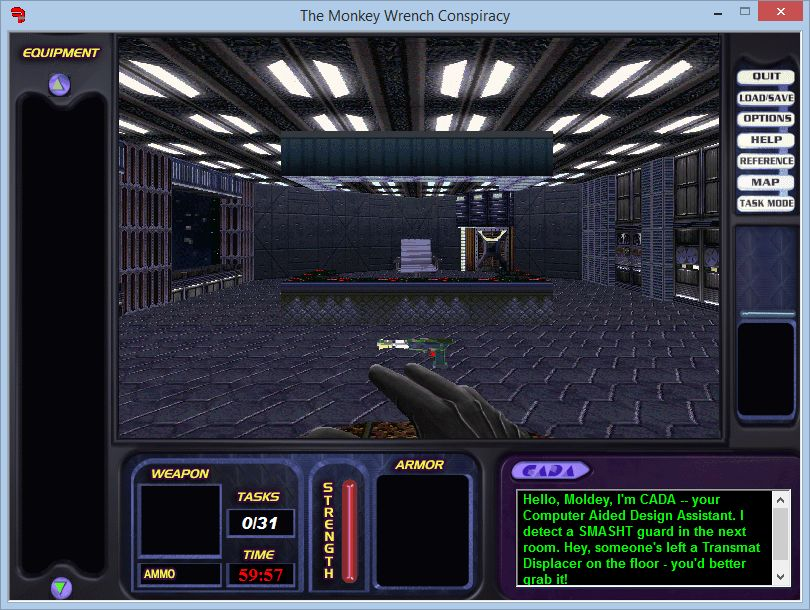
\includegraphics[width=0.6\textwidth]{figures/monkey}
    \caption{Screenshot of The Monkey Wrench Conspiracy}
    \label{fig:5}
\end{figure}

\begin{figure}[h]
    \centering
    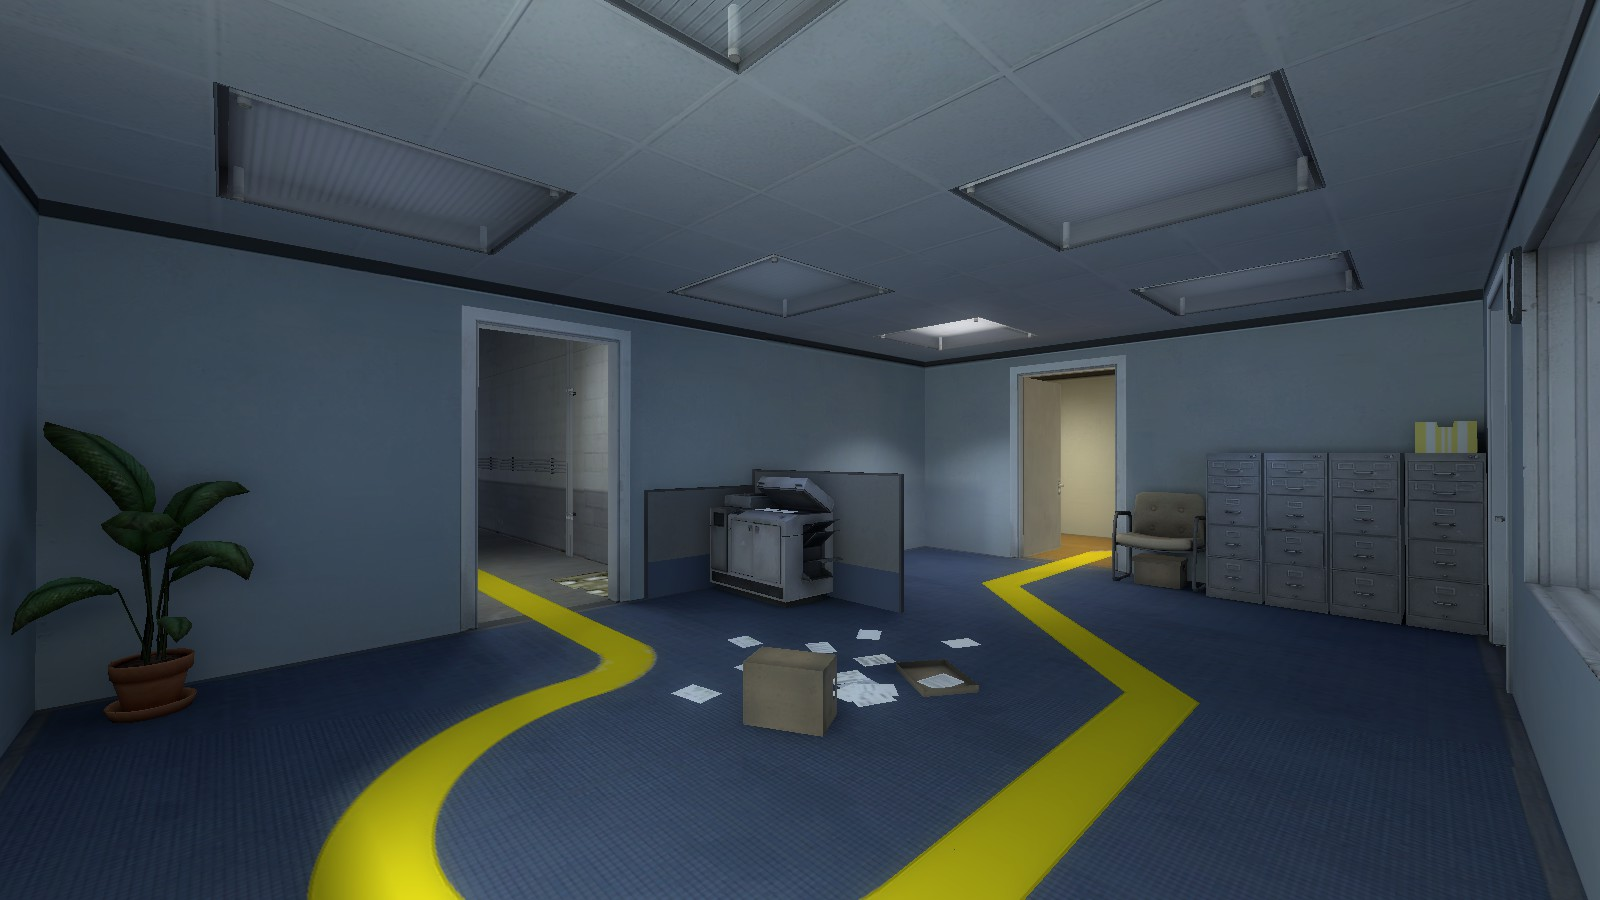
\includegraphics[width=0.6\textwidth]{figures/stanley}
    \caption{Screenshot of The Stanley Parable}
    \label{fig:6}
\end{figure}

\begin{figure}[h]
    \centering
    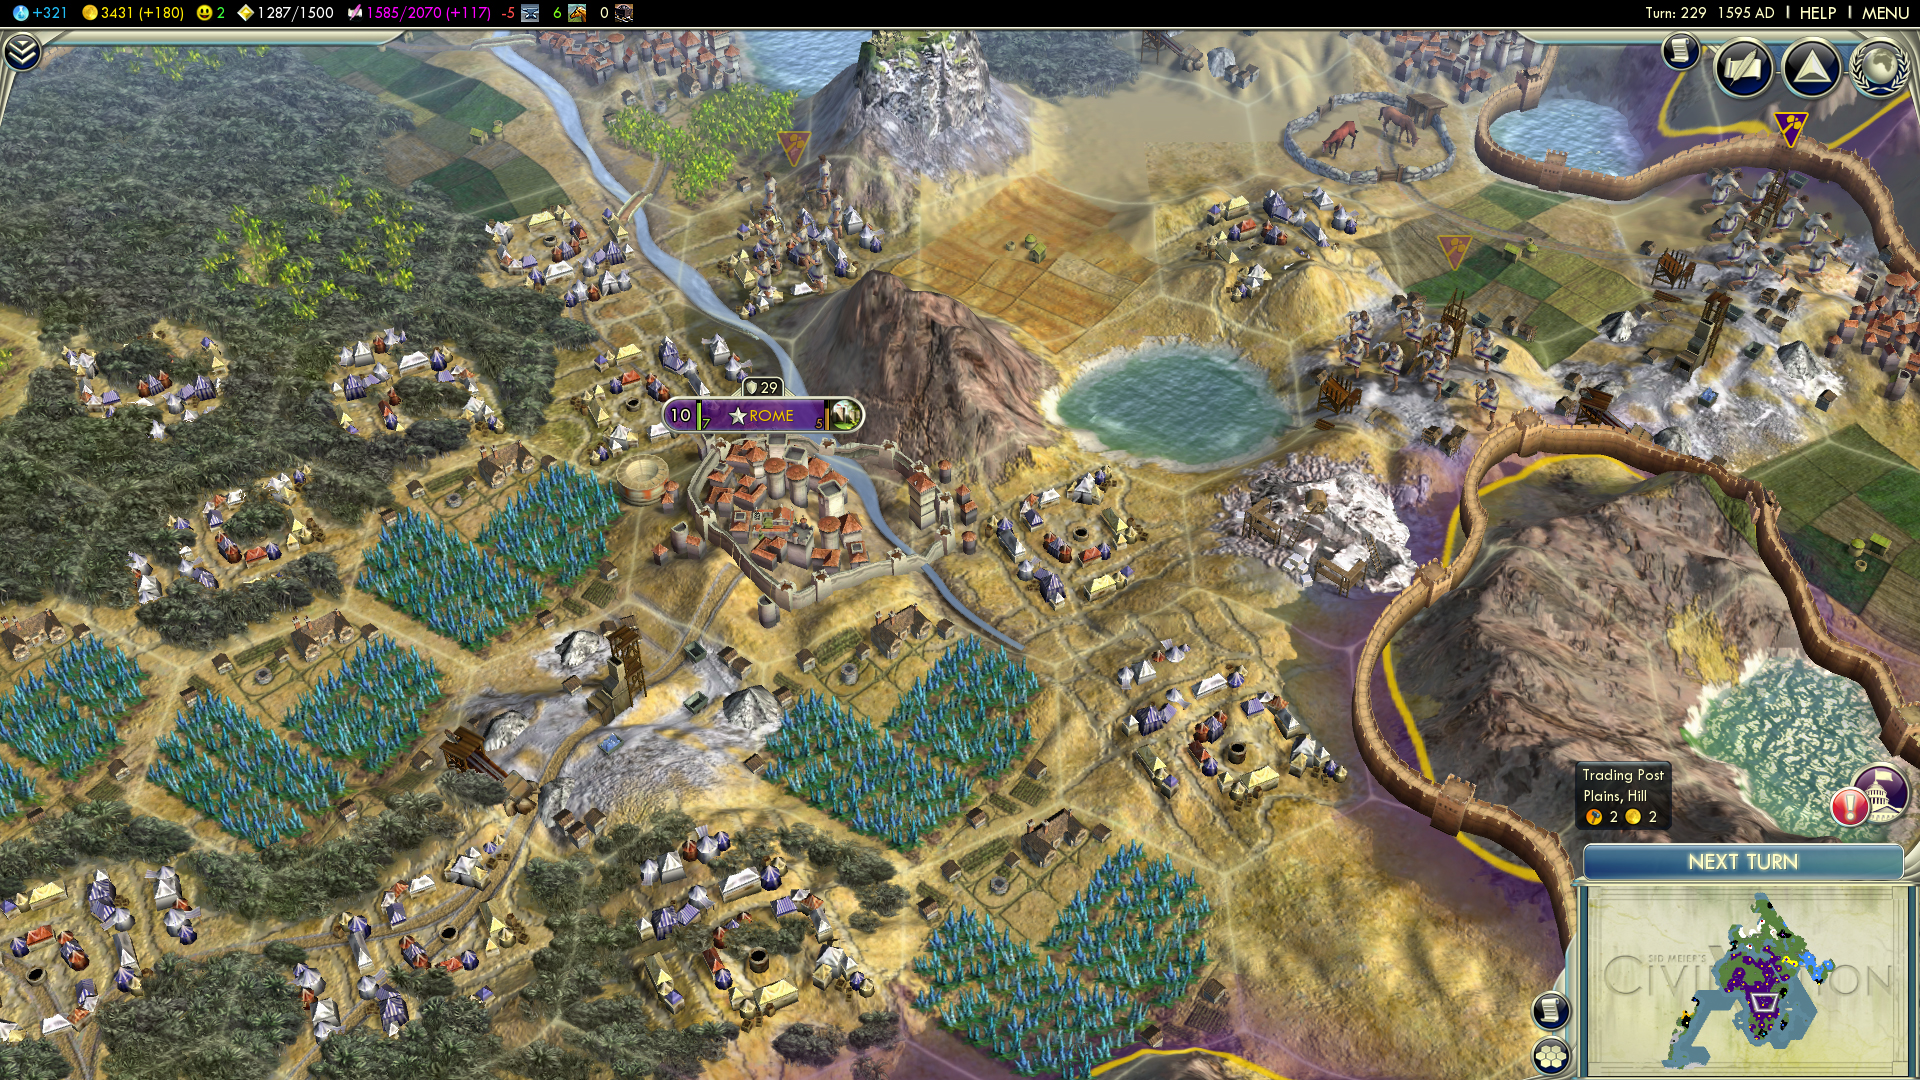
\includegraphics[width=0.6\textwidth]{figures/civil}
    \caption{Screenshot of Civilization 5}
    \label{fig:7}
\end{figure}


\chapter{The Basics of Gamification}

\section{The Benefits of Gamified Learning}
Video games have great potential in addition to their entertainment value.
There has been considerable success when games were designed to address a specific problem or to teach their players a certain skill \cite{compare}, which sparked interest to use more of this medium in regular instances of education.
Digital media and games in a teaching and learning context have been considered a valuable tool to engage students and make the learning process more interesting and motivating. Empirical research has shown that such games succeed in their goal to provide learning benefits \cite{framework} \cite{compare} \cite{domestic}.
games have always fascinated people in general \cite{aspects}, and due to the current generation of learners - mostly Millenials, Generation Z and Generation Alpha - being digital natives, which means they grew up with modern technology and are therefore already accustomed to digital games and content \cite{edu} \cite{domestic}, the further increase of such media being present in every context including the educational sector is the next logical step that can already be observed in day-to-day life.

Through simple educational tasks, studies have demonstrated that learning within a motivating setting improves learning outcomes and facilitate learning in general through enhanced engagement \cite{aspects} \cite{edu}.
Learning through gamification or other playful, mostly digital techniques gives a break from other more traditional teaching methods and embraces the motivational properties of such newer teaching frameworks. Studies show that digital games and media in general seem more attractive and enjoyable to students than traditional instruction through books or simply listening to a teacher speak \cite{compare} \cite{domestic}.

Old teaching methods have mechanisms that are no longer beneficial to students in the current day due to several reasons \cite{compare}.
Such reasons include but are not limited to:
\begin{itemize}
\item The methods do not encourage students to think outside the box or to find their own ways of coming to a conclusion since usually a very specific and rigid path to come to a solution is being taught \cite{compare}.
\item In school and other academic educational environments, the focus of the studies tends to be on the aquisition of good grades and on the passing of exams instead of encouraging the student to understand underlying concepts of the subject, which can lead to the student studying isolated topics very intensely just before an exam period and afterwards discarding the knowledge instead of integrating it effectively within their existing knowledge base \cite{compare}.
\item It tends to ignore the importance of integrating current and new trends of our society and culture into the educational environment, which causes a lack in authenticity in the assigned tasks and misses the realism that is necessary to allow students to be able and properly use the aquired skills outside of an educational context \cite{compare}.
\item Individual coaching and the organic adaptation of the learning material to cater to specific student needs is difficult to execute and non-existent in most educational contexts, especially for people with special needs. Although it is key in having a successful learning process, the rigidity of the current teaching methods make little room for this \cite{traditional}.
\end{itemize}

Generally, introducing gamification and Game-Based Learning in learning contexts renders the entire experience more fun which makes it more effective for most users \cite{aspects}.
Studies have shown that games in educational settings provide immersion, motivation and a high level of engagement as well \cite{framework}.
Besides just the fun-factor, several aspects of the learning process are being supported and reinforced which leads to increased effectivity.
Such aspects include:
\begin{itemize}    
\item The encouragement for intersectionality in the learning topic and/or process. Users are encouraged to combine knowledge from different areas of knowledge and expertise to choose a solution, make a decision or pick a way forward \cite{aspects}.
\item The freedom to test different outcomes or solutions to a problem based on the users decisions and actions, immediate feedback providing satisfying cues to continue trying and encouraging the exploration of different perspectives on the same problem \cite{aspects}.
\item In some instances, users are encouraged to contact other users or team members to discuss and negotiate what steps to take, which teaches and reinforces improvisation in tricky situations as well as social skills \cite{aspects}.
\item It promotes the users problem-solving abilities. Without the fear of severe failure, the user has the freedom to try out many different ways of solving problems, helping to create a more sound and solid approach to problem-solving tasks in the future \cite{compare}.
\item It equally promotes reflection and the exploration of the topic and of the user themselves, allowing them to progress at their own pace and take as much time as they need to repeat the different tasks and topics, creating a deeper space to integrate the learned themes \cite{engage}.
\item A platform for the users creative thought is provided and it creates a safe space to foster innovation without fear of failure \cite{compare} \cite{traditional}.
\end{itemize}

Gamification can create a mindset that encourages the user to try new things without suffering from a fear of failure and generally creates an enjoyable mental space and environment that promotes learning \cite{engage} \cite{compare}.
According to Gabe Zichermann, the use of game mechanics in the teaching of a new skill improves the ability of aquiring said skill by as much as 40\% \cite{edu}.
    
Additionally to reinforcing important skills such as the ones named above and the general learning of the subject matter, gamified and game-based learning teaches many other important skills and properties like digital fluency, automisation through repetition and general 21st century skills that are important for navigating the modern world \cite{framework} \cite{domestic}.
\newpage
\section{Game-Based Learning and Gamification}
There are many different types of games and game aspects that are combined with or used for education. Gamification and Game-Based Learning are often used as Synonyms for simplification purposes although they describe different strategies of using gaming for more than enjoyment purposes. Table \ref{table:1} is specifically comparing gamification and Game-Based Learning, but there are more keywords one may stumble across while researching in this field:

\textbf{Game:}
As a fundament to every other more specific type of games in skill or knowledge aquisition lies the question, what exactly is a game in the first place.
According to Merriam Webster \cite{fail}: 
\begin{quote} 
    A game is defined as: a. A form of competitive activity or sport played according to rules;
    b. An activity that one engages in for amusement; 
    c. (adj) eager or willing to do something new or challenging. 
\end{quote}
\indent
\textbf{Gamification:}
The definition of gamification is widely accepted as \cite{higher}: 
\begin{quote}
The use of game elements to create an active learning environment by engaging the learner in the process of knowledge acquisition.
\end{quote}
or as \cite{edu}:
\begin{quote}
The use of Game Mechanics, Aesthetics and Thinking to engage, motivate action, promote learning and solve problems.
\end{quote}
or just as \cite{higher} \cite{edu}:
\begin{quote}
The use of game design elements in non-game contexts.
\end{quote}
Gamification is inspired by video games and their ability to keep players engaged for long periods of time without losing interest \cite{equilibrium}. Through thorough analysis of what exactly makes games fun, developers isolate these aspects and apply them outside of gaming - for example in marketing, learning, or even in doing mundane tasks - to create a feeling of fun or even addiction to influence the users behaviour \cite{edu} \cite{fail}.
Although Gamification is also being used outside of educational or learning contexts \cite{compare}, game mechanics and gameplay elements are often applied to existing learning content.
Examples for such elements include: Achievement Badges, Points and Leaderboards, Progress Bars, Levels and Quests \cite{compare}.

\textbf{Game-Based Learning (GBL):}
Game-Based Learning or GBL for short uses games as part of the learning process \cite{compare}. Instead of trying to simulate an entire learning journey or enhance the experience thereof, Game-Based Learning isolates a single learning objective and turns it into a game.
The process for this can either be building new games from scratch to finetune it to the exact needs of this learning objective, or using existing games for educational purposes, a very common example for teaching economics and history is Sid Meyers Civilizations, see Figure \ref{fig:7}, that had been developed for non-educational purposes and was later refashioned into a learning game \cite{fail}. 

\textbf{Educational Games:}
Educational games are all games that are being designed and used with the intention to use them to teach and to learn \cite{compare}.
It tries to combine elements of fun and educational concepts with the goal of increasing student motivation and engagement \cite{compare}.
An educational game is built specifically with education in mind \cite{fail}. 

\textbf{Serious Games:}
Serious games are games designed for the specific purpose of training a group or individual for a specific task or job, not just for fun or entertainment, often used in medicine, military or for dangerous manual labor \cite{edu}.
A serious game possesses all game elements, it looks like a game, but it has a predetermined objective \cite{edu}. 

\textbf{Simulations:}
Simulations are similar to serious games but instead of just having a specific training purpose, they are made to simulate real-world situations and have the goal of offering the user a training environment that resembles real life \cite{edu}. 

\textbf{Game-inspired Design:}
The core of game-inspired design is the use of ideas and ways of thinking that are inherent to games and game development. It is not the use of game elements that defines this method, but rather the use of playful design in the final product \cite{edu}. 

\renewcommand{\arraystretch}{1.5}
\begin{table}[h]
\centering
\tiny
\begin{tabular}{ |p{3cm}||p{4.5cm}|p{4.5cm}|  }
\hline
\textbf{Comparison Points}& \textbf{GBL} & \textbf{Gamification}\\
\hline
Definition & - The use of games to enhance a learning experience & - The use of game design elements in non-game contexts \\
& - The use of a game to teach about a topic & - The use of game mechanics, aesthetics, and game thinking to engage, motivate action, promote learning and solve problems \\
& & - The use of game elements to create an active learning environment by engaging the learner in the process of knowledge acquisition \\
\hline
Purpose & - Teaching about one subject through a game & - Engaging and motivating the User to fulfill a task \\
& - Motivate students through gaming & - Turn the learning process into a fun experience \\
\hline
Benefits & - Skill-building through a cohesive game experience & - Very versatile, can be used in many different contexts \\
& - Keeps users motivated through ongoing action & - Better learning experience \\
& - Other benefits of general gaming like hand-eye coordination \& strenghtening decision making & - Motivates through Reward Systems \& Playfulness \\
\hline
Interaction with the Learning Process & - One learning aspect is isolated and taught & - The entire (learning) process is gamified \\
& - The learning goal is usually morphed to fit the game & \\
\hline
Use of game elements & - An entire game is used & - Game elements are selected and used to enhance the existing (learning) material / task \\
& & - Reward systems \\
\hline
Examples & - SimCity & - Duolingo \\
& - Sid Meyer's Civilizations & - Kahoot! \\
\hline
\end{tabular}
\caption{Comparison of GBL \& Gamification}
\label{table:1}
\end{table}
\newpage
\section{Intrinsic and Extrinsic Motivation}
\textbf{Intrinsic Motivation:}
The definition of intrinsic motivation has been described in many different ways but mainly follow the same core principle of it coming from the person itself, it comes from enjoying the activity or by having a large interest in it with little to no external influence \cite{corners} \cite{equilibrium}.
It is the pride one takes in doing the task, or the simple joy of the action \cite{domestic}, like an internal 'want to' drive \cite{equilibrium}.
Intrinsic motivation provides the reason for taking part in the game and is different than from what the gameplay demands \cite{mmo}.
Game designers and users alike favour intrinsic motivation due to it's fast pace and powerful feeling of reward, usually keeping players engaged longer \cite{corners}.
An example for an intrinsically motivated task within a game is the solving of a riddle to access a new area. The player isn't rewarded directly by the game but an internal feeling of a job well done motivates the player to forge on \cite{aspects}.

\textbf{Extrinsic Motivation:}
Extrinsic motivation can be defined as external reward or reinforcement \cite{domestic} or as a motivation to win in order to get a desirable reward \cite{corners}.
Examples for extrinsic motivation can be that a reward is given when the correct solution was provided \cite{mmo}, or the gaining of points to appear on a worldwide leaderboard \cite{aspects}. In many games, the slaying of monsters is rewarded with experience points or items, this also counts as extrinsic motivation \cite{corners}. Outside of the video game context, a student studying solely to earn good grades or to avoid failure, can also count as an instance of extrinsic motivation \cite{equilibrium}.
Despite it's short term effectiveness, relying solely on extrinsic motivation can cause some negative effects, as it tends to be very time consuming and a very unpersonal type of reward. Additionally, the rewarding feeling doesn't tend to last as long, which might dampen long-term motivation. Lastly, players set high expectations for themselves when extrinsic rewards are involved, leading to more negative thoughts towards loosing than normally \cite{corners}.

\textbf{Comparison:}
Intrinsic and extrinsic motivation often go hand in hand but differ in the fundamental drive that lays underneath. One could say that intrinsic motivation materialises in an "I want to..." drive, while extrinsic motivation materialises as an "I have to..." drive \cite{equilibrium}.
Often, by providing extrinsic rewards, intrinsic motivation might trigger as a concequence \cite{mmo}.

\textbf{Context in Games:}
Playing a game is often intrinsically motivated (the player wants to play the game) and the results are extrinsic (rewards inside the game give the player a feeling of success) \cite{domestic}.
Intrinsic motivation is widely seen as the most important educational aspect of digital games \cite{domestic} and is often used in more recent popular game genres to generate more enjoyment for the player on a short term basis \cite{corners}, although most games rather provide unrelated, extrinsic rewards due to it's easier implementation \cite{fail}.
Researchers agree that relying solely on extrinsic motivators does not create effective gamification \cite{equilibrium}.

\section{The Flow-theory}
The term "Flow" has become a very popular word, often used within the gaming industry. Flow is usually defined as a state of concentration so focused that it leads to absolute absorption in an activity \cite{higher}. Therefore, the "Flow Zone" is the zone where a person is engaged to the fullest \cite{mmo} and is therefore a very valuable and desirable state for game developers to have their games induce in their users.

Flow can come in many different forms, however a base set of behavioural patterns can be observed in individuals that enter a state of flow. These can include the ability to complete tasks, concentrate deeply, have clear goals, achive effortless involvement, to control one's actions, and have no concern for self or a sense of time during the activity. In short, it produces states of enjoyment represented by deep concentration on the activity \cite{higher}.

The state of flow, or flow zone is easily recognisable, but how is it induced? What are the conditions that need to be met for a person to enter such a state? A couple of strong motivators and triggers have been identified that could facilitate the entry.
Deep concentration can happen as a result of balanced but interesting challenges and use of skills, as well as a sense of control and satisfaction in the task \cite{engage} \cite{equilibrium}.
The activity needs to be sufficiently challenging and has a progression in difficulty to keep the user activated at all times \cite{higher} \cite{equilibrium}.
Clear goals at every step, immediate feedback, activities that merge action and awareness, a lack of distractions, no worry of failure or punishment due to failure are key factors that can help achieve Flow \cite{mmo} \cite{equilibrium}.
A mix of intrinsic and extrinsic motivators help the user stay engaged \cite{mmo}, a general intrinsic sense of reward can facilitate this even further \cite{equilibrium}.
In education, flow can be achieved through a combination of well-presented knowledge, interested students and stimulating teachers \cite{higher}.

In gamification, flow can be seen as a very important aspect of making the design work and effectively motivate the user.
The intrinsic characteristics of flow are argued to be present in gamification already, encouraging engaged and focused behaviour \cite{higher}.
In general, flow is an influential motivational theory often applied in gamification design and has frequently been used to create engaging, enjoyable experiences that captivate the users attention \cite{equilibrium}.


\chapter{Gaming Techniques for Effective Learning}

\section{Elements of Learning}
To provide a successful learning experience in and out of gamification, there are several factors that need to be taken into consideration. There are several approaches and sets of principles and goals that should be focused on to create a sustainable and productive learning environment, allowing for an effective acquisition of skills.

Unrelated to which medium is being used to teach the required skill, there are a few aspects that are key to teaching and should be integrated in the learning process to facilitate a fruitful learning experience:

\textbf{Acquisition of information and practice/repetition:}
First and foremost, providing the content for learning and practice is the key of any skill acquisition process. Study materials and a structure must be given to start any learning process in any environment to allow for the acquisition of information. Furthermore, the space for practice and repetition of the learned content helps integrate the gained knowledge in a more sustainable and permanent manner \cite{lifelong}.

\textbf{Ownership in learning process:}
Having the student actively partake in the shaping of the learning process encourages them to take ownership over their own process, allowing for more investment and motivation to learn the skill at hand \cite{aspects}.

\textbf{Adapted pace that allows reflection and thorough study:}
Allowing the student to move at their own pace increases the efficiency of the learning process and the process of skill acquisition as a whole. Having an adapted pace to the individuals needs allows for and encourages reflection and the possibility to study the topic thoroughly instead of being rushed through the lessons with minimal understanding or getting bored by too slow a pace \cite{online}.

\textbf{Social experience, collaboration \& relation to real life/relevant contexts:}
Authenticity is a major factor in successfully teaching a new skill. Embedding the learning within a relevant context and with relations to real life situations or having a simulation that alludes to it allows the student to integrate the new knowledge in a useful way that makes sense to them instead of learning said skill detached from reality \cite{aspects}.
Encouraging collaboration with other students within relevant learning processes can enhance the efficiency of learning. Through discussion with others, the topic gets integrated more thoroughly and additionally, it grants the student social experience and communication skills \cite{lifelong}.

\textbf{Training of problem-solving:}
Encouraging and allowing the individual student to tackle the posed problem or task and using their problem-solving skills is crucial to develop those skills further and can be used intersectionally and generally in life, not just the current topic of study. Getting better at problem-solving will further enhance the learning process and allow the student to come to some conclusions by themselves which provides them with a feeling of success and additional intrinsic motivation to continue studying \cite{lifelong} \cite{online}.

\textbf{Encourage multiple perspectives/intersectionality \& awareness of self and environment:}
For the better integration of the acquired knowledge or skill, the referencing of intersectional instances and encouragment to take on multiple perspectives on a topic will help the student think outside the box and create a wider network of knowledge for themselves as they are able to use the new information in a broader area, or even in contexts that were seemingly unrelated. Similarly, the knowledge or skills from other areas of expertise might support the student in learning this new particular skill. This generally enhances the students awareness of themselves as well of their environment, learning to look deeper than what is obvious on the surface and creating processes and connections that might have been overlooked otherwise \cite{aspects}.

\textbf{Progression \& facilitating success in the learning activity:}
In any learning environment it is important to have a visible sense of progression inside the process to keep the learners engaged and to facilitate success in the learning activity or respectively facilitate ongoing opportunities for a feeling of success within it to consistently show the students progress and motivate them further \cite{fail} \cite{equilibrium}.

\textbf{Assessment of progress:}
In traditional education especially but equally in any other learning medium, the assessment of progress is very important to further develop the learning process, to find out where more repetition is needed and which skills or topics have already been mastered. This allows for a more individual tailoring of the instructions or the following tasks to progress in the learning process and therefore a more effective path to acquiring the desired skill \cite{online}.

\textbf{Freedom to fail:}
Lastly, communicating to and showing that the student has the freedom to fail and the unhurried and non-judgemental space to try again in the case of failure is key to creating a non-hostile learning environment which encourages resilience and the willingness to keep trying even in the face of more complicated problems. This also encourages the exploration of different types of approaches, facilitating intersectionality, the taking of multiple perspectives as well as training the students problem-solving ability further \cite{fail}.

Games generally already embody a lot of these attributes, allowing for an engaging experience that can be translated to other teaching approaches. Some mechanics intuitively integrate processes and systems that appeal to the user, creating a motivating environment that fosters skill development due to the nature of those games as a whole, even in commercial contexts.

\textbf{Interaction:}
The core feature at any game and gamified tool or application in general is interactivity. For anything to happen or to move forward, the user is actively required to take action, take decisions and responsibility for setting their own pace \cite{framework}. This already tackles some main points of the learning principles listed above: Through the high adaptability of the process as a whole, the user takes ownership over the pace and part of the content, being able to spend more time on specific tasks that are of interest to them, making it more interesting and engaging.

\textbf{Structure \& Progression:}
Generally, games offer an inherent structure and clear path of progression, through their storylines, by completing puzzles or challenges, and are integrating those into a coherent context that makes the actions the player takes feel meaningful and keeps the player motivated to grow and improve further \cite{framework} \cite{fail}. Additionally, the progress tends to happen at the players own pace, allowing them to explore, come up with creative solutions that might help with solving future problems as well, and not feel overwhelmed by an externally enforced pace \cite{framework}.

\textbf{Challenge:}
Compelling tasks and challenging problems that provoke the players ambition and require at times complex problem-solving skills are a key aspect of many games today. Games have mastered the skill of creating those challenging problems while still keeping them doable, creating a pleasantly frustrating experience that highly motivates the players \cite{framework}.

\textbf{System thinking, changing perspectives \& intersectionality:}
Games generally require players to look at the bigger picture instead of isolated events or causes. This encourages them to look at a problem from different perspectives and try different approaches, potentially connecting the solutions to previous problems to the one at hand. Thorough exploration is at times not just encouraged but required instead of rushing through the game, allowing the player to properly wrap their head around the problem and potentially adapt their approach or even their goal \cite{framework}.

\textbf{Freedom to Fail \& room to change your mind:}
It is always possible to try again in games. When one approach to a problem doesn't work, players are encouraged to explore and find alternative ways to get to a solution. Some games are even centered around the idea of integrating failure into their game-loop, at times requiring the player character to die to get a certain outcome. This teaches resilience and that failure is not defeat, but the opportunity to learn something new and to adapt to new ways of doing things \cite{fail} \cite{framework}.

\textbf{Storytelling - hook \& induction into relevant context:}
Many games embed their puzzles and challenges into a broader context, usually facilitated by a storyline that is told one way or the other in the games world. Storytelling is a powerful tool to make the player feel engaged and interested in the task at hand, as well as to make the tasks and problems make sense within a context that doesn't feel detached or meaningless, inducing a more overarching sense of accomplishment than for example unrelated mini-games would \cite{fail} \cite{aspects}.

\textbf{Social thinking \& Team Work:}
Multi-player games often require players to work in teams, pushing them to think beyond their personal needs and goals, instead working together at times with strangers to find solutions and strategies to win the game, fostering social and group-oriented thinking as well as improving communication skills to quickly coordinate their team, and teaches them to think on their feet and improvise in sometimes high stress situations \cite{framework}.

\textbf{Provides clear feelings of success / Reward Systems:}
Games can clearly trigger intrinsic and extrinsic motivation in their players. Through different reward systems the user gets feedback on the completion of their tasks, keeping them entertained and engaged \cite{equilibrium}.

\textbf{Feedback:}
Additionally to the reward systems integrated in the games, there is generally a lot of feedback being given within the gameplay itself, providing the players with subtle direction that gives them a satisfying sense of knowing what they are doing \cite{framework}.

When developing a tool with the goal of effectively gamifying a learning process, it is crucial to keep those aspects and principles in mind. Gamification mechanics differ in a lot of ways from the mechanics in commercial or educational games, since instead of offering a whole, closed experience, the goal is to take an existing process, and add gamified mechanics and elements to it to make it more engaging and motivating. However, a lot of the basic concepts of these mechanics can be adapted for gamification as well.

\section{Design Elements}
Looking at design frameworks and elements with the goal to engage and capture their players from games in general and gamification as well as the connections between game elements and principles for engaged and effective learning show a lot of cross-over and allow for compilation into overarching aspects and game design elements that many authors seem to agree to be the key to sucessful game development for commercial games and gamification applications alike.

\textbf{Fantasy} or \textbf{Game Fantasy} is one of such core game elements, comprising not only the imagination of the player, but generally the scenario portrayed in the game material and the setting of it - refering to the environment that was built around the core mechanics of the game, giving it a believable context within the imaginary realm and help the player visualise it better \cite{aspects} \cite{model}. The knowledge that activity in the virtual space has no impact on the reality while the imaginary world captivates the player and makes them feel like nothing outside of it is relevant causes deeper engagement from the user, fostering interest in the activity and motivation to keep going, which increase the efficiency of learning environments through using this aspect within a gamified context \cite{aspects}.
It is important to note that despite the need for a convincing game fantasy, there has to exist a believable \textbf{relation to reality}. Games in their nature are often just enhanced simulations of real life activities, made more interesting by gamification techniques, but this is key in allowing the user to intuitively understand some ground rules about the world without needing a tiresome introduction \cite{lifelong} \cite{fail}.

Another important Game Element that is similar to and can go hand in hand with Game Fantasy is the \textbf{Narrative} within the game or gamified application. Briefly put, the game narrative is the description of happenings within the virtual space \cite{model}. Narrative Structures exist to provide immersion through storytelling within the game and allow the player to situate themselves within that world, enabling them to identify themselves better with the events that are happening as well as their player character \cite{lifelong}. Additionally, predictability is yet another aspect that a well thought out narrative structure may bring to the game, allowing the player to understand the imaginary world and it's machinations on a deeper level and learn to navigate it more intuitively. The gamified habit tracking and task management application Habitica (developed by HabitRPG, 2013) includes user oriented narrative through a role-playing game system, allowing the users to immerse themselves through the use of a personalised avatar and role-playing mechanics like a health bar and magic meter, as shown in Figure \ref{fig:3} \cite{avatar}.

\begin{figure}[h]
    \centering
    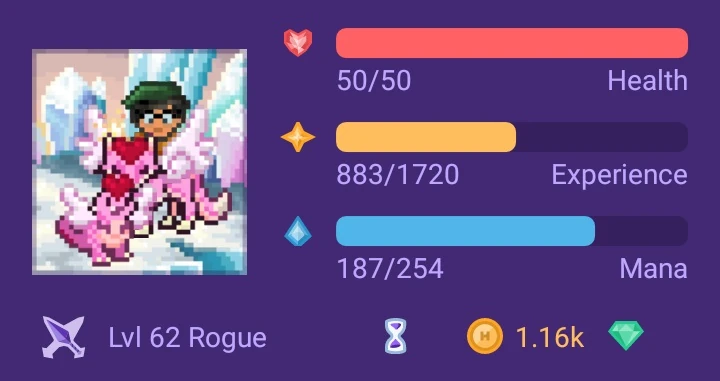
\includegraphics[width=0.7\textwidth]{figures/avatar}
    \caption{Player Avatar in Habitica}
    \label{fig:3}
\end{figure}

\textbf{Curiosity} is a key part of keeping a player interested and engaged with a game. Curiosity is what makes the player want to explore and learn more about the environment and the content of the game and what causes them to keep returning to play again. Games create a sort of second reality for the duration of play, with a set of rules that allows the player to explore and progress within the game, guiding them through the game world \cite{aspects}. The curiosity is triggered and sustained through continuously offering variety and novelty within the game, offering new information, narrative arcs, outcomes and general new elements that keep the player interested and on their toes \cite{engage} \cite{fail}. Offering the player a sense of mystery allows them to tap into their need to get to the bottom of the story or problem at hand, encouraging engagement and an intrinsic sort of motivation \cite{model}.

A recurring element that is found in every game or gamified application out there is \textbf{Challenge}. Challenge is provided through having appropriate levels of difficulty throughout the activity, as well as through progressively more difficult levels or given tasks that let the player work towards previously defined, meaningful goals, encouraging them to put effort into developing strategies and problem-solving to progress within the game \cite{aspects} \cite{engage} \cite{edu} \cite{fail}. The more personal importance the goals have to the player, the more ambition they will have to overcome the challenges given by the application, keeping them motivated \cite{model}. Therefore it is important to be aware of the amount of difficulty that is posed by the challenges. If the activity is too complex and hard to achieve, the player might feel disheartened and lose interest, while on the other hand, if the difficulty level is too low, the player might experience frustration and find the lack of challenge to be demotivating \cite{aspects}.
Especially within a learning context, increasing difficulty is key. Each consecutive task is expected to be more complex than the last, requiring the user to implement their previously gained knowledge and skills to solve the problem at hand \cite{edu}. The addition of new challenges in general is equally a way to coax the user into learning different aspects and new methods of application of the skill or topic they are currently striving to learn \cite{higher}.
Similarly, a game or gamified application should make the required skill \textbf{easy to learn but hard to master}. Through teaching the basics of the required knowledge to tackle the level at hand in simple terms but requiring mastery of this level before being allowed to move to the next, promoting deep engagement with a topic, motivating the user through challenging their understanding of it and rewarding them for successfully integrating the learned knowledge \cite{higher}.
This also fosters \textbf{replayability}, motivating the user to replay and re-engage with the level and the topic until they have proven their learning and understanding enough to progress \cite{fail}. In education and other learning environments, it is crucial to promote a cycle of multiple performances and repetition to allow the student to improve their skills and eventually reach their goal \cite{edu}. Here it is important to actively provide the conditions and opportunities to achieve said goals, using repetition primarily to encourage perseverance after an unsuccessful attempt instead of boring the student with the same subject and not enough new inputs to keep them engaged \cite{edu}. The language learning application Duolingo (developed by Duolingo Inc., 2012) uses a level-oriented system to teach their users, as can be seen in Figure \ref{fig:4} \cite{level}. Through gradual progression and mastery of the levels, the user unlocks the next, while also being allowed to return to previous ones at any time to deepen their skills.

\begin{figure}[h]
    \centering
    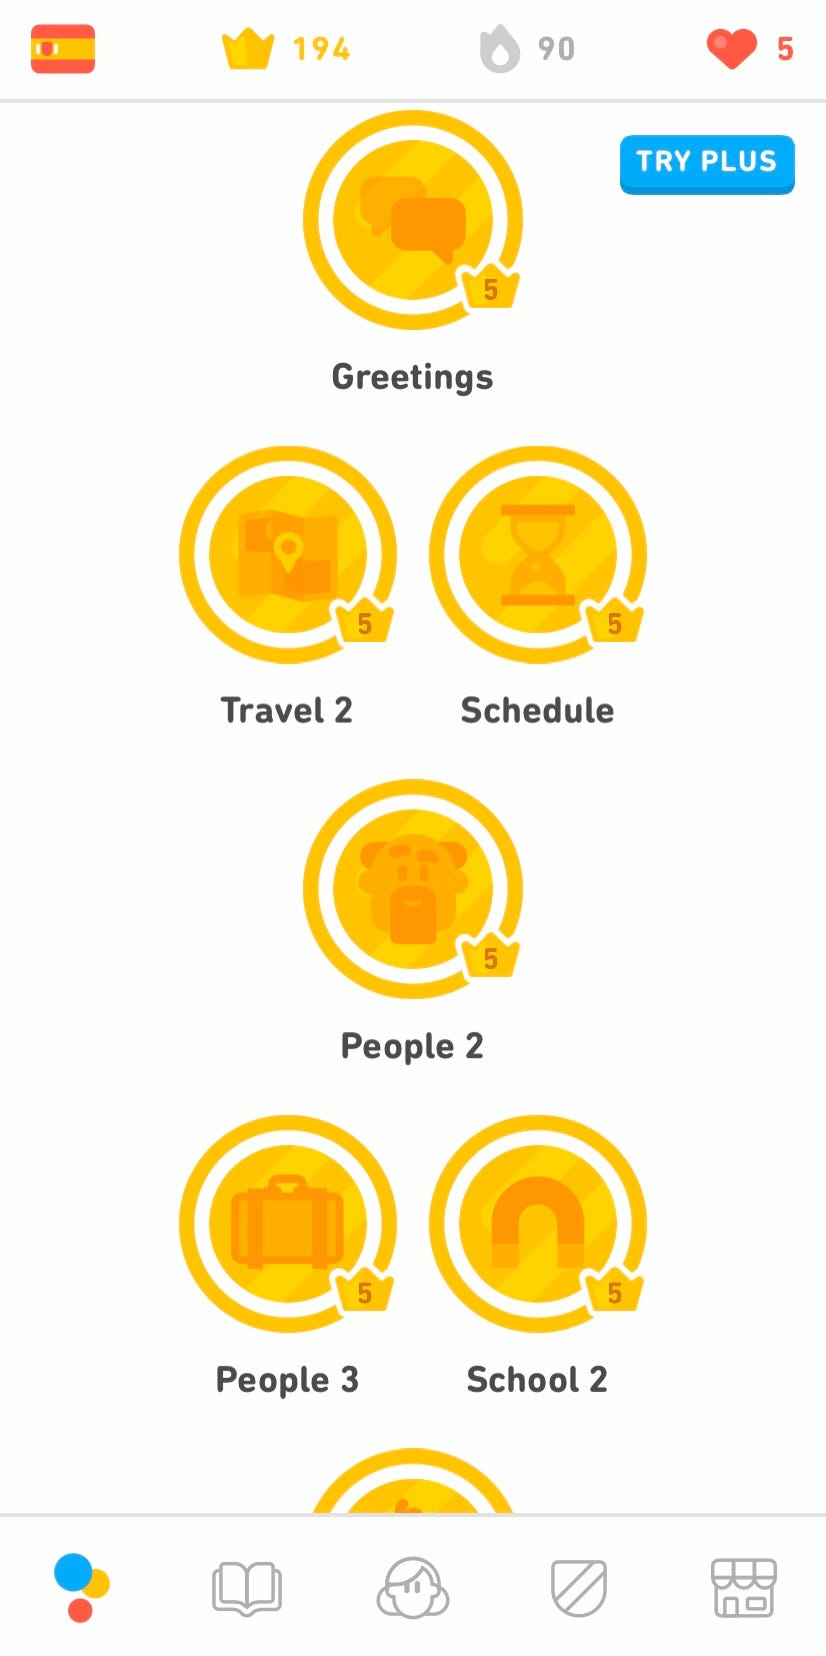
\includegraphics[width=0.37\textwidth]{figures/levels}
    \caption{Level Progression in Duolingo}
    \label{fig:4}
\end{figure}

The probably most important part of any game, gamified tool, or application are the users themselves. All users and players are active participants in the process, not just spectators. This distinctive feature found in all games is equally what plays a key role in gamification \cite{edu}. Inevitably it leads to another main element found in all games and effective learning processes and gamification tools: \textbf{Interactivity}. The more interactive the experience, the more engaging it is \cite{higher}. Interaction means that the players actions trigger events or responses from the application that are related to their immediate manipulations \cite{model}. Another type of interaction that is often present within games is through the affiliations with others. This can be an interaction with a non-player character within a roleplaying game \cite{engage}, or interactions between players, directly or indirectly. This might require direct communication with other players, but is most often used in the form of \textbf{Competition} and \textbf{Collaboration} with others \cite{model} \cite{higher}.
In multiplayer games, collaboration between players can often provide them with a mutual benefit that is very desirable, putting the players who do not play as part of a team at a noticeable disadvantage \cite{lifelong}. This can be through the collaboration within a battle, to the sharing of resources.
While collaboration is a game aspect that some people enjoy, competition usually stays the main motivator and driving force of a game \cite{lifelong}. In a gamified context, competition usually means the comparison of skills, progress and successes to peers and strangers. This can happen in direct confrontation like in the gamified quizzing tool 'Kahoot!' (developed by Kahoot! ASA, 2013) where the participants go head to head in a battle of knowledge, or through comparing in-game statistics like points, badges, their ranking in leaderboards or the amount of achievements in order to gain recognition \cite{higher} or to just feel the satisfaction of having beaten other competitors.

Adjacent to competiton with others is the \textbf{Competition with self}. Through the option to repeat a level for example, the user can compare their performance with their previous try, thereby competing with themselves \cite{fail}. This gives them the possibility to assess their own skill-level and performance, and provides the tools to improve. It is often seen as a very crucial part of any learning process, since the ability to see their own improvements is extremely motivating and rewarding, especially if it is visible in an obvious and continuous manner \cite{lifelong}. Just as in competition with other players, a scoring system can be introduced to visibly keep track of the users progress \cite{lifelong}. A less intrusive way of introducing numbers and visuals to track the individuals progress is for example through experience points or levels.
In the same vein, providing ongoing feedback about their progress and giving general affirmation about the users successes and performance incentivizes them to challenge themselves and perform even better \cite{higher} \cite{engage}.

Generally, users want to feel in \textbf{control} of their own experience and to have the \textbf{choice} and \textbf{freedom} to shape it according to their needs. Control is given to the player by making them feel like their actions have direct and significant concequences \cite{aspects}. This makes them feel valued and empowered and simulates relative freedom of action and freedom of choice, allowing them to move at their prefered pace and doesn't impose on their autonomy \cite{engage} \cite{model}.
A flexibility to select different paths or approaches to the same problem or task can go a long way to make the user feel in control as well \cite{higher}.
Additionally to promoting the feeling of the player being an active part in shaping the process and development of things, the option of \textbf{multiple paths} to reach a goal is fostering the development of a diverse and intersectional skillset, allowing the user to build their own strategies and approaches which is a key characteristic of active learning \cite{edu}.

The \textbf{freedom to fail} is crucial in games, gamification and learning environments alike. This describes the protection from negative concequences for initial failures \cite{engage} which allows the user to explore the topic at their own pace without needing to worry about getting the best results right away, motivating them to seek different approaches to the same task, branching out with their problem-solving skills and gives them the opportunity to thoroughly interact with the subject before moving onto the next one \cite{lifelong}.

Any activity in games and learning should be achievable and reasonable. Especially within an educational environment, the tasks should be adapted to the users pre-existing skill and potential to offer an individual and effective learning experience \cite{edu}. In gamified applications as well, the \textbf{feasibility} of the content is key to provide a positive experience. Through clear communication in the application about what tasks need to be completed and which problems need to be solved \cite{engage}, and through implementing a concise and simple on-boarding process that equally lowers the barrier of entry to start using the application, the process of interaction with the app stays convenient and low effort, which promotes fidelity to using the application regularly, as well as general motivation and feelings of success and progress within the individual \cite{fail}.

Providing \textbf{goals} within the game or learning process is crucial as it dictates the entire content of the application as well as what kind of experience it will be for the user \cite{model}. Users will pursue the goals through interacting with the tasks and problems, gathering the needed items, information, knowledge, etc. that is required to advance within the framework of the game or gamified process. The more focused and clear the goals are, the more engaged the player will be and the easier it will be for them to feel intrinsically motivated \cite{engage}. The goals of the game or application can either be at the end of it, marking the completion of the entirety of the process, or can also be split up into sub-goals that each comprise a topic or task or even just a section of said task to complete. This way, feelings of success can be spread out throughout the entire experience, providing notable rewards or events every time such a goal is reached, fostering ambition and motivation in the user and further creating an effective experience \cite{lifelong}.

Stimulating \textbf{Emotions} and general \textbf{Sensations} of the users is key to providing a satisfying and appealing experience. This refers to the use of visually pleasing graphics within the application, keeping them consistent and simple enough to not overwhelm the user \cite{fail}, as well as to other stimuli for the senses like effective sound design and general appropriate media presentation of the product \cite{model}. Through creating visual or auditive feedback within gamified applications that reward the user after a good performance in a fun and humouristic way, the creation of strong emotions can be stimulated and supported, leading to more engagement, as well as enhance the general enjoyment of the process \cite{fail}.

And last but not least, \textbf{Rewards} are usually the most straightforward and efficient way to foster motivation within the users. Through well thought out rewards that the user considers helpful in their quest to advance within the process, extrinsic motivation can be triggered which usually is a very powerful motivator for many individuals. This ranges from rewards for completing levels, for using the app for multiple days in a row or for getting a new high score \cite{fail}. The most common rewards are elements such as points, badges, achievements or a higher place on a public leaderboard.
The next chapter will dive further into different types of reward systems and different motivators that can be used to keep users engaged.

\subsection{Negative Use of Game Elements in Gamification}
Despite the many positive effects that game and gamification elements can have on their users, with the wrong type or the wrong amount of game mechanics implemented in the application, it can turn unmotivating or even frustrating.

A lot of games and gamified applications use leaderboards or other form of competition with either strangers, friends or both to motivate the user and increase replay value, creating incentives for the user to log on again the next day. While this might seem like an effective way to create engagement, the downside can be a forced sense of social obligations. The user might feel pressured to go online and do their daily challenges to not fall behind on the leaderboard, or feel peer pressure to partake in recurring events with their friends \cite{mmo}, potentially even making the user feel threatened if the competition with others is mandatory, especially if said competition is with co-workers or friends and family \cite{lifelong}. A good example of the use of leaderboards in a gamified context is the language learning application Duolingo (developed by Duolingo Inc., 2012), see Figure \ref{fig:1} \cite{leaderboard}. In the worst case this can create a dynamic like any other forced routine in day to day life, playing the game or using the app starts feeling like work or a chore, which either will cause unnecessary stress or will cause the user to stop using it eventually \cite{mmo}.

\begin{figure}[h]
    \centering
    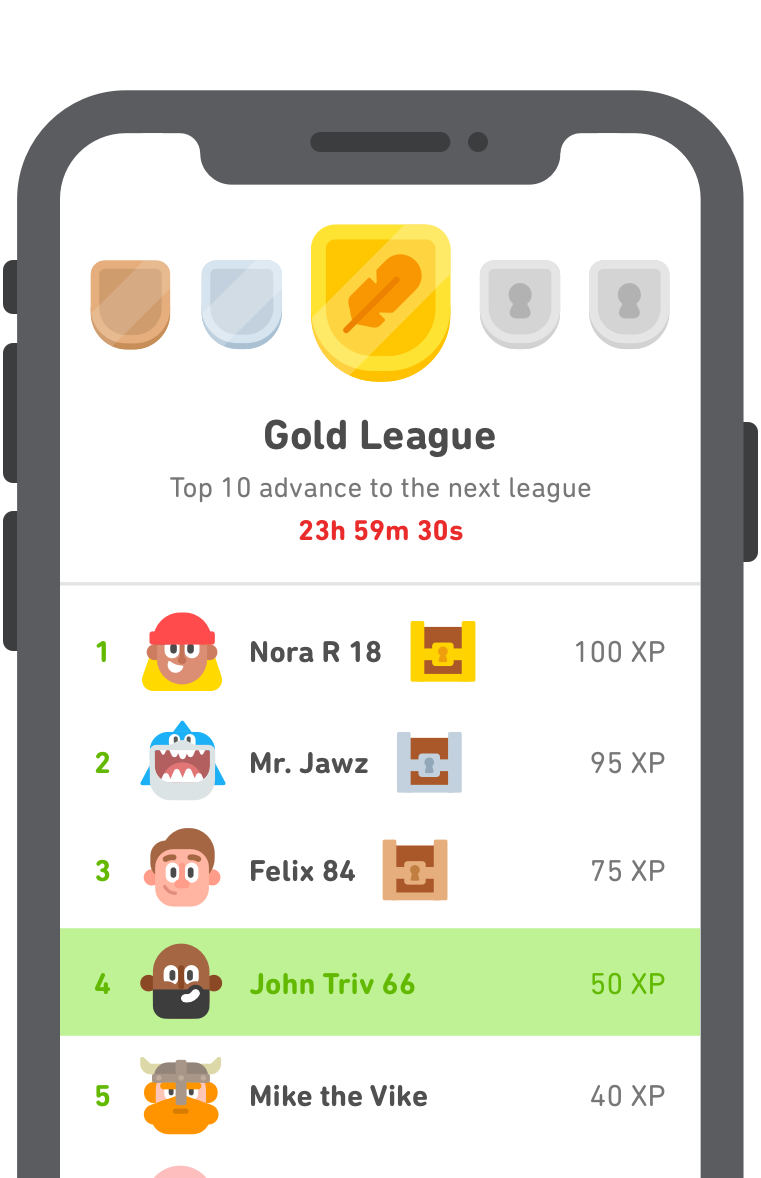
\includegraphics[width=0.48\textwidth]{figures/leaderboard}
    \caption{Leaderboard in Duolingo}
    \label{fig:1}
\end{figure}

Even without the social aspect, there might be systems in place that aim to motivate the user to come back, but trigger stress and negative reactions instead. Commonly, log-in streaks are used to reward the player for their commitment, but some applications dish out penalties instead if a day is missed, creating yet another cycle of frustration for the player. Once again, a good example of this is the application Duolingo which aims to motivate their users to return through a streak system, as can be seen on Figure \ref{fig:2} \cite{streak}.

\begin{figure}[h]
    \centering
    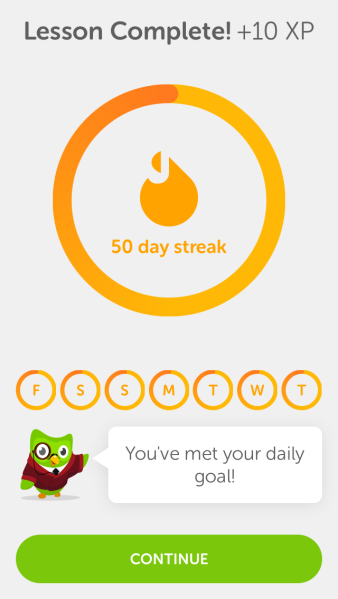
\includegraphics[width=0.46\textwidth]{figures/streak}
    \caption{Streak System in Duolingo}
    \label{fig:2}
\end{figure}

Well designed reward systems are powerful tools that are used within games or gamification to create a sense of success and progress, motivating and engaging the user or even inducing a state of flow, but not always do they trigger these feelings, instead promoting negative reactions if used improperly \cite{equilibrium}.

Shallow gamification heavily relies on extrinsic rewards to motivate their users instead of working on triggering the users intrinsic motivation, most notably through systems like points and badges. This may initially create engagement, using immediate gratification to keep the experience fun and stimulating, but it fails to maintain this engagement, making the user lack the necessary long-term investment in the activity that it takes for habits to be formed and goals to be achieved \cite{equilibrium}.
The reason why excessive use of extrinsic rewards hamper especially the users own intrinsic motivation can be explained by the paradox of the 'Overjustification Effect'. It has been observed that initially motivated individuals, which then recieve extrinsic rewards for the activity they have been doing previously, lose interest in this activity when those rewards cease to be given. The motivation for participation shifts from inherent enjoyment of the activity to the expectation for the next external reward, overshadowing any previously existing intrinsic motivation. The sole reason to keep partaking in the activity becomes the hunt for the next dopamine kick that the reward triggers \cite{equilibrium}.

The excessive use of rewards in gamified contexts also can come across as controlling, causing the user to feel less competent and like they are not in charge of their own process, equally decreasing intrinsic motivation.

While reward systems are an important part of making gamification work, using them too generously is more likely to backfire than to actually help the user to stay engaged. This seems to be commonly disregarded in the development of current gamified applications and might be why those gamification tools are failing today \cite{equilibrium}.

\section{Reward Systems}
Reward systems are the most important design element for any game and especially any gamified application. They keep the users engaged and motivated, appealing to their sense of ambition and need for affirmation. Previously, the concepts of intrinsic and extrinsic motivation were defined and analysed, most reward systems build on top of that knowledge and aim to trigger said kinds of motivation.

One reward system that has been proposed is called 'The Three corners of Reward' \cite{corners}. It divides the different types of rewards into three archetype categories, explores how to combine these for efficient use, and analyses their interactions with each other. The main three categories are personal reward, material reward and competitive reward.

\textbf{Personal Reward:}
The players already go into the game with their own ideals and goals that are the main reason they are playing the game for. These goals are personal to the player which makes them volatile and therefore hard to study and define well, however certain core values can be extracted and observed. These core values usually are for example ambitions to unlock something inside the game, or the completion of the game.

\textbf{Material Reward:}
A material reward is a reward given for the players actions, and for their successful behaviour in game. The player obtains something they want after putting time and effort into playing the game, this often is an item, experience points or temporary improvement that gives them an advantage.

\textbf{Competitive Reward:}
The competitive reward is often described through the satisfaction after besting another player. This can mean getting a higher score, a quicker time, beating other players in battle or just having a higher score of completion in the game.

Most often, games offer a combination of these types of rewards to trigger different types of motivations within the player, namely intrinsic motivation, extrinsic motivation and social play as a motivator.

\textbf{Personal/Material:} 
The interaction of these reward systems result in triggering intrinsic motivation within the player. It promotes genuine enjoyment in the activity and creating a large interest to play in the player with little to no external influence. The enjoyment comes from personal aspects and the game becomes more meaningful to the player. This increases the better the player gets at the game. This type of reward is generally favoured due to its fast pace and is often used in recent popular game genres to create enjoyment on a short term basis.

\textbf{Material/Competitive:}
The interaction of the material reward and competitive reward results in enhanced social play motivation. It offers ways for players to connect and play with others in a multiplayer environment. This increases the general competitiveness of the players as well as the overall time spent playing the game.

\textbf{Personal/Competitive:}
Personal and competitive rewards combine to create extrinsic drivers to keep the player engaged. It is a motivation to win in order to receive an outcome. This could for example be scoring well on a public leaderboard, since this would be viewed as an attractive position to dedicated players. However, extrinsic rewards are usually very time consuming to achieve and tend to be unfocused in which kinds of players they appeal to, making it important to not rely on this area alone to keep the players engaged. The rewarding feeling tends to not last as long as the other types of rewards, which can further be unappealing to players. It also happens that players create high expectations for themselves, resulting in more negative thoughts and feelings towards potential failure than usual.

Another system suggests to not just differentiate intrinsic and extrinsic motivation but offers more concrete aspects within extrinsic motivation, separating them further into underlying types. These include the following \cite{equilibrium}:

\textbf{External Regulation:}
External regulation is defined as the least autonomous form of extrinsic motivation. The main driver and motivator here is the obtaining of a reward, or the avoidance of a penalty. Players engage in the demanded behaviours to maximise the pleasure of recieving an external reward and to minimise the chance of recieving punishment for a failed task. Points, badges and leaderboards can be used to motivate the user in that regard, promoting engagement in the task at hand.

\textbf{Introjected Regulation:}
Internal pressure like guilt or shame is a very powerful motivator for people. Introjected regulation relates to this feeling of pressure to motivate the user. The actions and tasks that need to be completed are still imposed externally, however the source of pressure and therefore motivation comes from the user themselves. Gamified systems are capable of harnessing this by using simple mechanisms like the common and well known 'Streak'-system as presented in Figure \ref{fig:2}, generating the internal pressure within the user to keep logging in each day to maintain this streak and can act as a powerful motivator to promote continued use of the application.

\textbf{Identified Regulation:}
A more autonomous form of extrinsic motivation is identified regulation. In this type of motivation, the user individually recognizes the value of the promoted behaviour and accepts that motivation as their own. This happens when the users personal goals are aligned with the goals of the application, for example learning a new skill that they need to learn for personal purposes. Gamification can shape the given experience within the gamified tool to match these personal goals, although that requires a good grasp and knowledge about the user base.

\textbf{Integrated Regulation:}
Integrated regulation is the most autonomous form of extrinsic motivation. When the individual users general life goals and their identity aligns with the goals of and desired behaviour asked by the gamified application, a very deep and powerful motivation can be formed. If motivation like that can be achieved, it fosters deeper engagement and mastery of the subject at hand. By promoting general skills that align with the users overarching goal and personal development, for example in creativity or problem-solving, gamification can help reach that level of profound engagement.

Besides just systems that aim to narrow down the types of rewards and how to properly make use of them in game development and the development of gamified applications, there also are more specific rewards that are commonly given within games and have proven themselves to be successful \cite{mmo}.
Experience point Rewards are a universal way of keeping players motivated and ignite their ambition to keep playing and improving in the game. This is usually portrayed through an experience point meter that shows how many more the player needs to accumulate to advance to the next level. This goes hand in hand with another popular reward, namely Unlocking Mechanisms. Through for example gathering experience and advancing within the game or application, new parts of the game can be accessed, like new maps, new levels or new item rewards, that were previously inaccessible. Through this method, a curiosity within the player can be maintained about what might be made available in future play, keeping them motivated to keep on playing.

New items themselves as rewards are yet another popular method, rewarding the player with in-game material depending on the effort and risk that was taken. These items can be more or less valuable or useful, motivating the player to keep seeking out this reward to get a potentially even more epic item.
Resource rewards are similar to item rewards but differ in one key aspect, as they are only a temporary support in the game or application. This can be a one time use health potion to replenish the users hearts or a power up that temporarily improves the abilities of the player character, or grants more experience points for a certain duration. The mechanism of motivation is the same.

The most immediate way to provide a reward is through feedback messages. After the user achieved something inside the application, those messages are directly displayed on the screen, giving an immediate sense of reward and achievement. This can happen through colorful pop-ups that congratulate the player on their success, or in games even through positive reaction of a NPC (Non-Player-Character). Despite the praise being generated by a computer and not coming from an actual human, this still affects human emotions and behaviours, working further to drive the user to complete their tasks.

Rewards like the ones named above are easy to implement and are specifically triggering extrinsic motivation, but there are some ways to trigger intrinsic motivation within the players as well \cite{mmo}.

Transparency around rewards like experience points, unlockable skills and items, and the ability to showcase them to other players creates comparison and therefore competition. This can trigger an inner sense of pride and ambition within the individual players, making them more likely to put more effort into the task at hand.
The reward system has to be viewed as fair and equal to all players. This can be facilitated through the aforementioned transparency, as well as through keeping track of the players advancements in the application, suggesting that there are no hidden ways or shortcuts to recieve the rewards and reach the goal. The keeping track of the successes and advancements of the player itself can equally keep the player motivated, reminding them of past achievements and urging them to forge ahead.
Chance has always been a factor in games that keep the players curious and engaged. If a reward does not have a 100\% chance to be given, players have the tendency to keep trying until the wanted reward is recieved and the thrill of the unknown is keeping them engaged.
In the same spirit as chance, scarcity in rewards triggers the feeling of greed and need for the unlikely reward within the player. Nothing is gained for free,  and the player has to take sizeable risks or efforts to aquire the rare reward. Like in the material world, items that are associated with rarity, like gold, are desirable and people will go to considerable lengths to acquire it.
Giving constraints like these make it more likely for the player to feel a sense of intrinsic motivation, prompting them to keep on playing and engaging with the available material \cite{mmo}.

Generally, there are some base guidelines around implementing reward systems in games and especially gamified applications to motivate users to start and keep playing. The most important aspect to keep in mind is that rewards should be accessible during shorter play sessions. Giving the user feelings of success early on is crucial to promote replayability and make the user more likely to keep logging back in as it lowers the hurdle to start playing \cite{mmo}. If rewards are held off too long, the player might get frustrated and feel obligated to keep playing for a longer time to achieve what they want, which can lead to them abandoning the game due to feelings of stress and pressure.
Competition is yet another point that needs to be very carefully considered, along with the goals the application offers as well as the emotions that it is meant to elicit. This is such a difficult aspect due to the vast variety of natures amongst players, who all value those aspects differently and might have differing reactions to the different uses of these mechanics. Overall, players seem to be more interested in rewards that lead to gaining more power or skills in game than in pure aesthetic items meant as a trophy. As such, rewards that are useful for the advancement in the process are more effective to motivate the users, like power ups, unlocking levels and similar rewards \cite{fail}.
A scoring system overall is an easy way to introduce a transparent system to keep track of ones own progress and successes, allowing the player more ownership over their process as well as keeping them motivated. This can be as complex or as simple as desired, ranging from 'success or no success' to more complicated point systems where a score is obtained through different actions or in different gameplay areas, creating a much more detailed image of the players progress \cite{lifelong}.
As aforementioned, humans give objects different values based on their scarcity. Therefore, a reward for an 'excellent' success or display of behaviour should be rare enough to be valuable without it accidentally triggering frustration and demotivation on the players side through it either being too complicated to achieve or simply be too scarce \cite{lifelong}.

Especially when it comes to reward systems and motivators in gamification specialized for skill acquisition, it's important to remember that the learners themselves usually are their own main motivator with quite some initial intrinsic motivation already present. Through careful choosing of what motivators and rewards to use, this can be amplified to create an engaging learning experience, however this initial motivation can decrease quickly if the player discovers too many disadvantages or sources of frustration within the application, causing them to get bored or to feel overwhelmed \cite{lifelong}. Instead of bombarding the users with many rewards in the hopes to keep them satisfied, it is key to use the available methods smartly and in the necessary instances and instead of overwhelmedness trigger healthy ambition and a sense of pride in the users individual achievement.

\section{Aspects to watch out for in Development}
There are many pitfalls in the design and development process of a gamified application for personal learning purposes. These can mostly be compiled into the following categories: the differences between learning in the classroom and individual learning; game design versus instructional design; the target demographics of the application; and general learner motivation and needs.

Learning within a controlled classroom environment, be it at school, university, or similar, is very different from learning by yourself from home. Due to the 2020 pandemic, many people had to switch to online learning and several issues have been observed, mainly the lack of motivation or the inability to properly self-motivate, as well as a lack of structure \cite{online}. A teacher provides a schedule, a system to learn, support when needed, and the presentation of the learning materials. All this needs to be substituted skillfully so the user does not feel overwhelmed or lost and can profit from an effective learning process.

This leads to one of the main issues within the development of gamified instructional material. The design of these tools needs to balance pedagogical requirements and learning aspects with the fun-factor of games to function effectively, which is difficult as even in commercial game development triggering that notion of fun for the player while gaming can be tricky \cite{online}.
Often, gamified tools for learning are either designed by a team of instructional designers, or a team of game designers, but rarely both. Studies show that for successful development, both game designers and educators are needed to contribute good and engaging game design but also good pedagogy, otherwise the resulting product will neither be fun nor motivating, and additionally lacking in the application of key principles that facilitate effective learning \cite{framework}.

Demographic dependence is another big aspect to keep track of in the development process. It is important to know what target group you are catering to and what their individual needs are. Those demographic groups can include but are not limited to: gender, age, ethnicity, social background, disability, and generally minorities and disadvantaged communities.
Age and gender for example play a major role in which gamification mechanics specifically are efficient and well recieved \cite{fail}. For instance, competition and competitive play is differently recieved between people of different genders, regardless of age. Goals and appeal to emotions have different importance for different age groups, as well as the reception and motivating factor of different types of rewards.
Depending on the purpose of the application and its users intended social environment, gamification tools need to be adapted to those differing needs as well. If the tool is designed for the use in the workplace, specifically for larger companies, competitive elements that promote competition between co-workers might rather be percieved as a stress factor and even as threatening instead of motivating \cite{lifelong}. If the tool is designed for private use, some friendly competition with registered friends can go a long way in motivating the user instead of being a stressor.
It is important to research previously conducted studies about the preferences and psychology of the target demographic that the application is aimed at to get a good grasp on what approach to take in the style of gamification which should be used in development.
Like in any other medium, but especially in educational and learning contexts, the representation and portrayal of minorities and disadvantaged communities is a sensitive subject and a hard terrain to navigate. Discrimination because of race, gender, disability, or social status is increadibly common and sometimes done not out of malice but out of lack of knowledge about these topics. It is important to be mindful and respectful of the differences and needs of these groups, especially if no developer that is part of the affected groups is part of the team \cite{engage}. Again, research is of utmost importance to create an inclusive and welcoming learning environment, also within gamified learning tools.

Lastly, paying attention on how to properly captivate the users attention and foster motivation and engagement through gamification mechanics is key. Being overzealous in the use of gamification aspects can end up being more harmful than effective. The quality of motivation is much more important than the quantity of it \cite{equilibrium}. Therefore, understanding nuances between intrinsic and extrinsic motivation, how to trigger them, and the strengths and weaknesses of both those approaches, is crucial to use them effectively in the design, development, and implementation of the gamified tool. It is important to keep in mind the 'Overjustification Effect' as well - the paradox that when extrinsic rewards are provided for intrinsically motivated activities, intrinsic motivation decreases \cite{equilibrium}. Thorough reflection on which rewards and motivators are being used is necessary to create a successful gamified learning experience.

It is important to keep in mind that not all kinds of rewards and gamification mechanics work for all learners and for all learning outcomes. Being aware of the target group and of the ultimate goal for which the gamified application is being developed will provide the required insight to choose the right game elements to utilize \cite{framework}.
Solely focussing on flow theory may not guarantee the wanted outcomes in learning and habit building, it is needed to apply additional motivational frameworks to achieve the desired result \cite{equilibrium}. Instead, finding a good balance between challenge and skill encourages the neglect of distractions and helps foster concentration, engagement and enjoyment, which in turn can also trigger Flow \cite{higher}. The level of difficulty has to be variable enough to adjust to the individual users abilities and needs to avoid a negative impact on their motivation, allowing them to succeed and keep progressing all while maintaining a healthy degree of pleasantly frustrating challenge that triggers the users ambition \cite{model}. Walking the line of keeping the application sufficiently challenging while not making it too demanding or stressful can be difficult, although it is crucial to not make the user percieve the usage of it as work or as unenjoyable \cite{mmo}.

The so called 'BPL Gamification' is a gamification system often refered to as 'Pointification' by experts in the field and refers to the shallow gamification technique of using badges, points and leaderboards to create an externally appealing combination of game elements and is wrongly assumed to make the product immediately more engaging by applying it to a process \cite{equilibrium}. This process of arbitrarily rewarding users with points and similar items is massively overused and not very effective in most cases. In the worst case, such poorly applied game design elements can undermine a learners innate motivation to partake in an activity and sabotage the initial goal of using gamification in the tool that is being developed. Instead it is recommended to implement deep gamification techniques, focusing beyond the superficial focus on extrinsic rewards, to foster an immediate sense of gratification in the user and additionally offer effective long-term learning outcomes.

Not falling into the trap of desiring to benefit from the positive effects and outcomes of gamification without putting in the proper time, research and effort to develop a strategy fitting to your own project is the path to a successful gamified product, since according to many empirical findings, a simple BPL approach is not enough for creating an effective gamified experience \cite{equilibrium}.


\chapter{Conclusion - Do's and Don'ts of Gamified Elements in Personal Learning}
Having looked at, and compiled much data all about gamification and other gaming techniques, as well as aspects that are crucial to effective learning, there are some Do's and Don'ts for the design of an effective gamified application for skill and knowledge acquisition that have crystalized. As with the development, it is key to be very clear and aware of the purpose, intended content and target group of the application that is being developed, but generally these guidelines apply. Finally, a couple of questions can be asked that can serve as a useful guideline during the development process. For a compiled overview, reference Table \ref{table:2}.

\section*{Do's} \indent
\textbf{Relevant \& Accessible Rewards:}
Well thought through rewards that match the users needs and help them progress. This refers to external rewards within the application that are useful to the user in the near future, such as a power-up for example. Exceptional performances should earn a bonus reward. These rewards should equally be accessible during short play sessions. \\ \indent
\textit{Why:} Through using relevant rewards that are tailored to the target group, and their needs and psychology, extrinsic motivators are firstly more effective, and secondly might help trigger intrinsic motivation within the user. Similarly, offering more exceptional rewards for a good performance motivates the user to strive for improvement, therefore making the learnings more effective. Allowing the user to feel rewarded and successful even during short play sessions hightens engagement and the likelyhood of the user returning more frequently.

\textbf{Storytelling \& Immersion:}
Implementing some sort of narrative within the application, either through the actual telling of a story or through situating the content of the application within a fictuous context. Additionally, to enhance immersion, it is possible to provide some sort of roleplay or fictious interactions for the user within the application or even allow for the creation of an avatar or similar virtual incarnation for the user to identify with. \\ \indent
\textit{Why:} Through storytelling, the application may engage the users on a deeper level, making them interested in finding out what is next or what else can be explored. This game design element can even trigger deeper intrinsic motivation within the user which is beneficial to effective learning. The use of an avatar can be a good choice to further make the application feel like play, permitting the user to immerse themselves further and therefore have a personal connection with the content, equally fostering engagement and an intrinsic drive.

\textbf{Well designed Graphics \& Audio:}
Visually pleasing assets and a cohesive, overarching graphic design for the application with a friendly, direct, and easy to understand interface. Simple but effective sound effects for feedback. \\ \indent
\textit{Why:} A visually appealing application is more likely to be used and to remain continuously used. Good visual design as well as a simple design for the overarching game interface increases the satisfaction of interacting with the app and avoids frustration with the handling of the application itself. The concious use of satisfying sound effects increase the feeling of success when recieved and further make the application usage fun and stimulating.

\textbf{Feedback \& Affirmation:}
Similar to rewards, providing immediate feedback for the users performance and actions, keeping the application responsive to interactions and help users keep track of their progress and improvements. \\ \indent
\textit{Why:} Giving the user immediate feedback after their actions will help motivate and guide them through the content of the application, and implementing for example a scoring system to track their achievements and progress helps fostering confidence in their improvements and keeping them engaged. Additionally, having audiovisual cues when a task is completed or a goal achieved is a satisfying reward for the user, increasing the fun-factor for the task and therefore the application as a whole.

\textbf{Interaction \& Levels:} 
Design the application with many levels, either for tasks, stages of knowledge, skill levels, etc. Additionally, achieve a high density of interaction through interactive tasks and step by step completion, making the user a participant and not an audience. Gradually allow the user to gain access to the next steps, for example unlocking new levels or introducing new mechanics. \\ \indent
\textit{Why:} Completing a level is a big motivator for users. Separating larger tasks and topics into smaller, more easily digestible parts and creating levels around it will keep the user engaged, entertained and motivated through the feeling of success they get by finishing a level. Making those levels as interactive as possible not only keeps the users attention but also facilitates learning through direct contact with the topic instead of just absorbing information. The gradual unlocking of content will keep the user curious as to what might come next and will make it more likely for them to keep on using the application.

\textbf{Well defined Goals:}
Provide concrete, feasible short, medium and long-term goals. Be very clear about what is expected from the user and how to achieve the set goal. Especially in a learning context, set clear, realistic learning objectives. If possible, make the goals in the application align with the personal goals of the user. \\ \indent
\textit{Why:} Clear direction in what to do helps the user feel secure in their actions and gives them a clear prospective on the process and goal they are supposed to achieve. Implementing milestones as short and mid-term goals helps measure progress and improvements, motivating the user to keep going while giving them the feeling of success they need to feel like they achieved something relevant for their own personal development. Especially if the application is tailored to a specific need or want of the user, for example, to learn a language the goals can be aligned with their own and therefore provide a strong internal drive.
Clear and transparent goals also prevent frustration that can arise from dealing with a task or topic that is too complex and seemingly without an end to it.

\textbf{Clear Rules and Parameters:}
Provide a very transparent set of rules and parameters as well as a clear and efficient onboarding to instruct the user on how to use and progress within the application properly. \\ \indent
\textit{Why:} Not knowing how exactly an application works and having the rewards and feedback feel arbitrary very quickly triggers frustration and will demotivate the user. Having clear instructions on what to do will help the user achieve the goals better and faster while also helping them comprehend the content more easily.

\textbf{Challenge \& Increasing Difficulty:}
Create sufficiently challenging levels or tasks that over the course of the progression within the app become more difficult, staying synchronised with the increase in skill and knowledge of the user. Depending on the content and if it is compatible with different degrees of difficulty, having adjustable difficulty levels can be beneficial for the user. Additionally, make sure the user can repeat the tasks and levels at their own leisure. \\ \indent
\textit{Why:} A consistent sense of challenge that is still reasonable and manageable can encourage the ambitions of the users, keeping them motivated to compete further with themselves by solving increasingly complex problems and giving the satisfaction of completing them. Furthermore, increasing difficulty is needed to have an efficient learning process, gradually introducing new knowledge and providing the tools for the user to acquire said knowledge and excel at it. Making repetition available will give the user the opportunity to revise knowledge and deepen their understanding of the topic.

\textbf{Novelty \& Variety:}
Provide new content regularly, offer different types of playful learning and not just memorization excercises. Switch up the type of interactions regularly. \\ \indent
\textit{Why:} If the content and the interactions stay the same, the user will loose interest due to boredom. This also does not promote learning as the content stagnates. Providing different methods of acquiring the knowledge and switching them up will keep the user engaged and curious, as well as foster their adaptability and problem-solving skills.

\textbf{Choice \& Exploration:}
Promote decision making by offering a flexible path selection, allowing exploration and giving the user the power to set their own pace. Allow the user a certain freedom of deciding what task, problem, or level they want to tackle next. \\ \indent
\textit{Why:} Giving the user a certain amount of autonomy within the process encourages them to take control of and feel responsible for their progress without feeling pushed or restricted by the application. Being able to choose the next step and the content they want to engage with will encourage motivation and circumvent the reluctance that the user might feel if the path the application offers is too rigid and might make uninteresting content unavoidable and a barrier to move forward. Allowing users to set their own pace in learning equally prevents them from feeling overwhelmed and encourages them to keep trying and eventually progressing.

\textbf{\emph{Situational:} Optional Social Interaction:}
Have opt-in elements for social play within the application like leaderboards, a friendlist, the forming of parties, etc. \\ \indent
\textit{Why:} Some people strive with social factors within the applications they interact with. This is highly individual and only recommended if it is very clear which target group the application is developed for and how their stance is on this type of interaction. Make sure to research thoroughly before implementing this.

\section*{Don'ts} \indent
\textbf{Changing Rules:}
The sudden change of rules and parameters that have been a certain way for the entire process up until that moment, but suddenly are different for no apparent reason. \\ \indent
\textit{Why:} If suddenly the ruleset changes, it is disorienting to the player. They might not understand why and how exactly the existing rules were discarded or adjusted, and might have a difficult time adapting to the new circumstances. Frustration might arise as a concequence and hamper motivation and engagement. \\ \indent
\textit{What to do instead:} Design and communicate a clear ruleset at the beginning that will not change throughout the process.

\textbf{Too overwhelming or not stimulating enough:}
The tasks or levels are either too easy or too difficult. Too much new content is introduced at once. The onboarding is too long and complex. \\ \indent
\textit{Why not:} If the tasks or levels are too easy, the user will quickly feel understimulated and feel a lack of challenge, which will lower their ambition, get bored and decrease their motivation to engage with the application. On the other hand, if the tasks are too difficult or too overwhelming by, for example, introducing too much new information at the same time, the user might feel helpless and lost within the task, or get frustrated by not achieving the necessary goals to progress. Additionally, the first hurdle within the application is the onboarding process. If it is too difficult to understand and takes too long to explain, the user will loose interest right away and might cease to use the application before even having properly explored it. \\ \indent
\textit{What to do instead:} Have a good balance of well designed tasks, building on previously gained knowledge to permit the user to solve it without too much difficulty while still introducing new content bit by bit, providing a comfortable level of challenge. Keep the onboarding concise and clear.

\textbf{Restrictive path \& pace:}
Rigid structure of how a task is to be completed without much room for exploration or alternative methods. Needing too much repetition of one task or level before allowing the user to move on to the next or not allowing any repetition at all. \\ \indent
\textit{Why not:} Designing the structure of the application in a very rigid and restrictive way might make the user feel caged and forced to do things a certain way without giving them the opportunity to take a little control over their process. This mostly just leads to frustration and reluctance to continue as the dictated path and pace might not be compatible with the learners individual needs. Through too much repetition the user will get bored, while allowing no repetition at all might not give the user enough time to properly integrate the subject. \\ \indent
\textit{What to do instead:} Allow a selection of a few levels or tasks that can be tackled next instead of forcing a specific one. Let the user decide whether they want or need to repeat the task or level before moving on to the next one, and allow them to return to the level and re-play it at any moment.

\textbf{No Feedback on Progress:}
Lack of progress bars, levels, any measurement of performance and progress. \\ \indent
\textit{Why not:} If no means are given to the user to keep track of their own achievements and progress, there is no possibility to notice improvements or advancements, taking away a crucial motivator. Additionally, a lack of indicators about the users score or ability doesn't offer a way to allow them to compete with themselves, therefore not fostering the ambition within the user to perform even better in the next task, or by repeating the same level. \\ \indent
\textit{What to do instead:} Implement a very transparent system that allows the user to keep track of their skills and knowledge improvements.

\textbf{Bad Reward Systems:}
No rewards are given at all. Too many rewards or rewards that are unrelated to the application or to the tasks the user needs to complete. Too much focus on extrinsic motivators or competitive rewards. Only using badges, points and leaderboards as a reward system. \\ \indent
\textit{Why not:} Poor quality rewards do not achieve the motivational boost within the user that is required to create an engaging experience. Rewards that are unrelated to what the user is currently doing and have no actual use within the application except cosmetic are proven to not foster motivation and might even frustrate the user. Badges, Points and Leaderboards, while perhaps initially motivating, do not provide long term motivation and therefore users might loose interest very fast. Similarly, if only extrinsic rewards are given without a system to help promote intrinsic motivation in the user as well, users are less likely to stay driven and engaged. \\ \indent
\textit{What to do instead:} Give rewards that matter and are useful to the user, for example unlocking further levels or power ups that give them a temporary boost or advantage within the application. Try to find ways to foster intrinsic motivation through well designed external rewards and other feedback.

\textbf{Punishment for Failures:}
Loss of a life, health, points or similar when a level or task is failed. General punishment for not performing well. Loss of advantages through not maintaining a daily log-in streak. \\ \indent
\textit{Why not:} Failure in itself is already a stressor for users, if the application amplifies that feeling of failure through negative consequences, users might feel demotivated, frustrated, disappointed in themselves, and might put less effort into working with the application or stop using it completely. Showing that failure is not something bad and can be seen as an opportunity to try again and get better is key in providing an effective and healthy learning process and therefore this kind of negative feedback should be avoided. \\ \indent
\textit{What to do instead:} Give incentives to try again. Give rewards for repeating a failed level. Give rewards every time the user logs in and do not take them away when they fail to do so.

\textbf{Obligatory Social Interactions \& Competition:}
Competitive elements like leaderboards or direct battles, as well as other social elements like mandatory participation in parties or guilds or having to play with friends as fixed component of the gamified application. \\ \indent
\textit{Why not:} While some forms of competition and social play can be quite motivating for some people, most will perceive it as stressful and demotivating, especially if the user might not have as good a high score or performance as others, showing them their lack of skill as a lower spot on the leaderboard or similar. Social play that comes in the form of daily interactions that are either mandatory or would give a massive disadvantage if missed can cause the user to start perceiving the usage of the application as a chore or as work since they are required to log on every day or suffer penalties. Neither is good for fostering motivation or engagement. \\ \indent
\textit{What to do instead:} If a social component has to be present, keep it optional and opt-in. Let the users decide if they want to compete or otherwise interact with strangers or with friends.

\textbf{Time Limits:}
Imposing time limits on the completion of the levels or tasks or similar. \\ \indent
\textit{Why not:} Most people percieve a time limit as stressful and it will impact their performance negatively. Although this method is effective for some people, it is safer to leave out this specific game mechanic. \\ \indent
\textit{What to do instead:} Allow the user to set their own pace. Set limits to how many actions can be taken to make a problem or task more challenging, if any.

\section*{Questions as Guidelines for Development}
\begin{itemize}
    \item What are the specific goals that the gamified tool is supposed to achieve?
    \item What behavioural goal is the focus? Increased motivation, engagement, enjoyment or improved achievement?
    \item Are there experts on the team for the content of the application (eg. Instructional Designers)?
    \item What is the target audience and how does that impact the choice of game elements?
    \begin{itemize}
        \item Learning styles, characteristics \& preferences
    \end{itemize}
    \item How can the knowledge about the future users be leveraged to cultivate their intrinsic motivation?
    \item Which extrinsic rewards are useful and effective for the purpose of this application?
    \begin{itemize}
        \item Are the quality of rewards favoured over the quantity of them?
    \end{itemize}
    \item What is a fitting, satisfying visual style for the application?
\end{itemize}

\renewcommand{\arraystretch}{1.5}
\begin{table}[h]
\centering
\small
\begin{tabular}{ |p{7cm}|p{7cm}|  }
\hline
\textbf{DO'S} & \textbf{DON'TS}\\
\hline
\begin{itemize}
    \item Relevant \& accessible Rewards
    \item Storytelling \& Immersion
    \item Well designed Graphics \& Audio
    \item Feedback \& Affirmation
    \item Interaction \& Levels
    \item Well defined Goals
    \item Clear rules and parameters
    \item Challenge \& Increasing Difficulty
    \item Novelty \& Variety
    \item Choice \& Exploration
    \item \textit{Situational:} Optional Social Play
\end{itemize} &
\begin{itemize}
    \item Changing Rules
    \item Too overwhelming or not stimulating enough
    \item Restrictive path \& pace
    \item No feedback on progress
    \item Bad Reward System
    \item Punishment for Failures
    \item Obligatory Social Interactions \& Competition
    \item Time Limits
\end{itemize} \\
\hline
\end{tabular}
\caption{Do's and Don'ts for implementing Game Elements in a Gamified Learning App}
\label{table:2}
\end{table}

\newpage
\thispagestyle{empty}
\newgeometry{left=-0.615cm,right=0cm,top=0cm,bottom=0cm}

\includegraphics[height=\paperheight]{figures/Poster_img}

\restoregeometry

\chapter{Outlook \& Future Work}
Despite quite some research that has been done in the field of games and gamification in education, there is a clear lack of well defined guidelines and design elements specifically for gamification in personal education, especially for usage in private contexts, outside of school or other educational environments. 

Recent events have reshaped the learning landscape, the results of which will only be well evaluated in a few years. The 2020 pandemic has forced individuals and institutions to adopt new ways of learning and teaching, both for professional and personal growth. Thanks to previous experiences, new methodologies and different combinations of methodologies are being applied, leading to diverse results. New studies will need to observe the outcomes and update what we know about gamification techniques in the learning process.

\newpage
\bibliographystyle{apacite}
\bibliography{main}

\newpage
\thispagestyle{empty}
\newgeometry{left=3cm,right=3cm,top=8cm,bottom=3cm}

\Large
\textbf{Declaration of Authenticity}\\

\small
\noindent
I declare that I completed the Bachelor thesis independently and used only these materials that are
listed. All materials used, from published as well as unpublished sources, whether directly quoted or
paraphrased, are duly reported.
Furthermore I declare that the Bachelor thesis, or any abridgment of it, was not used for any other
degree seeking purpose. \\

\vspace{2cm}
\noindent
Berlin, 20.02.2024
\hfill

\includegraphics[width=0.3\textwidth]{figures/Signature}
\\
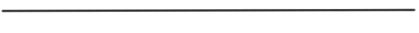
\includegraphics[width=0.3\textwidth]{figures/Line}
\hfill
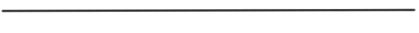
\includegraphics[width=0.3\textwidth]{figures/Line}
\\
\noindent
Place, Time 
\hfill
Signature

\newpage
\thispagestyle{empty}

\begin{center}
    \begin{figure*}[!b]
        
\includegraphics[width=0.3\textwidth]{figures/HIVE_Logo} \\
        \\
        \\
        
\includegraphics[width=0.3\textwidth]{figures/GD_Logo} \\
        \\
        \\
        
\includegraphics{figures/HTW_Logo}
    \end{figure*}
\end{center}

\thispagestyle{empty}
\addtocounter{page}{-1}
\newgeometry{left=-0.615cm,right=0cm,top=0cm,bottom=0cm}


\includegraphics[height=\paperheight]{figures/Cover_Back}

\restoregeometry

\end{document}
